% Options for packages loaded elsewhere
\PassOptionsToPackage{unicode}{hyperref}
\PassOptionsToPackage{hyphens}{url}
%
\documentclass[
]{book}
\usepackage{amsmath,amssymb}
\usepackage{iftex}
\ifPDFTeX
  \usepackage[T1]{fontenc}
  \usepackage[utf8]{inputenc}
  \usepackage{textcomp} % provide euro and other symbols
\else % if luatex or xetex
  \usepackage{unicode-math} % this also loads fontspec
  \defaultfontfeatures{Scale=MatchLowercase}
  \defaultfontfeatures[\rmfamily]{Ligatures=TeX,Scale=1}
\fi
\usepackage{lmodern}
\ifPDFTeX\else
  % xetex/luatex font selection
\fi
% Use upquote if available, for straight quotes in verbatim environments
\IfFileExists{upquote.sty}{\usepackage{upquote}}{}
\IfFileExists{microtype.sty}{% use microtype if available
  \usepackage[]{microtype}
  \UseMicrotypeSet[protrusion]{basicmath} % disable protrusion for tt fonts
}{}
\makeatletter
\@ifundefined{KOMAClassName}{% if non-KOMA class
  \IfFileExists{parskip.sty}{%
    \usepackage{parskip}
  }{% else
    \setlength{\parindent}{0pt}
    \setlength{\parskip}{6pt plus 2pt minus 1pt}}
}{% if KOMA class
  \KOMAoptions{parskip=half}}
\makeatother
\usepackage{xcolor}
\usepackage{color}
\usepackage{fancyvrb}
\newcommand{\VerbBar}{|}
\newcommand{\VERB}{\Verb[commandchars=\\\{\}]}
\DefineVerbatimEnvironment{Highlighting}{Verbatim}{commandchars=\\\{\}}
% Add ',fontsize=\small' for more characters per line
\usepackage{framed}
\definecolor{shadecolor}{RGB}{248,248,248}
\newenvironment{Shaded}{\begin{snugshade}}{\end{snugshade}}
\newcommand{\AlertTok}[1]{\textcolor[rgb]{0.94,0.16,0.16}{#1}}
\newcommand{\AnnotationTok}[1]{\textcolor[rgb]{0.56,0.35,0.01}{\textbf{\textit{#1}}}}
\newcommand{\AttributeTok}[1]{\textcolor[rgb]{0.13,0.29,0.53}{#1}}
\newcommand{\BaseNTok}[1]{\textcolor[rgb]{0.00,0.00,0.81}{#1}}
\newcommand{\BuiltInTok}[1]{#1}
\newcommand{\CharTok}[1]{\textcolor[rgb]{0.31,0.60,0.02}{#1}}
\newcommand{\CommentTok}[1]{\textcolor[rgb]{0.56,0.35,0.01}{\textit{#1}}}
\newcommand{\CommentVarTok}[1]{\textcolor[rgb]{0.56,0.35,0.01}{\textbf{\textit{#1}}}}
\newcommand{\ConstantTok}[1]{\textcolor[rgb]{0.56,0.35,0.01}{#1}}
\newcommand{\ControlFlowTok}[1]{\textcolor[rgb]{0.13,0.29,0.53}{\textbf{#1}}}
\newcommand{\DataTypeTok}[1]{\textcolor[rgb]{0.13,0.29,0.53}{#1}}
\newcommand{\DecValTok}[1]{\textcolor[rgb]{0.00,0.00,0.81}{#1}}
\newcommand{\DocumentationTok}[1]{\textcolor[rgb]{0.56,0.35,0.01}{\textbf{\textit{#1}}}}
\newcommand{\ErrorTok}[1]{\textcolor[rgb]{0.64,0.00,0.00}{\textbf{#1}}}
\newcommand{\ExtensionTok}[1]{#1}
\newcommand{\FloatTok}[1]{\textcolor[rgb]{0.00,0.00,0.81}{#1}}
\newcommand{\FunctionTok}[1]{\textcolor[rgb]{0.13,0.29,0.53}{\textbf{#1}}}
\newcommand{\ImportTok}[1]{#1}
\newcommand{\InformationTok}[1]{\textcolor[rgb]{0.56,0.35,0.01}{\textbf{\textit{#1}}}}
\newcommand{\KeywordTok}[1]{\textcolor[rgb]{0.13,0.29,0.53}{\textbf{#1}}}
\newcommand{\NormalTok}[1]{#1}
\newcommand{\OperatorTok}[1]{\textcolor[rgb]{0.81,0.36,0.00}{\textbf{#1}}}
\newcommand{\OtherTok}[1]{\textcolor[rgb]{0.56,0.35,0.01}{#1}}
\newcommand{\PreprocessorTok}[1]{\textcolor[rgb]{0.56,0.35,0.01}{\textit{#1}}}
\newcommand{\RegionMarkerTok}[1]{#1}
\newcommand{\SpecialCharTok}[1]{\textcolor[rgb]{0.81,0.36,0.00}{\textbf{#1}}}
\newcommand{\SpecialStringTok}[1]{\textcolor[rgb]{0.31,0.60,0.02}{#1}}
\newcommand{\StringTok}[1]{\textcolor[rgb]{0.31,0.60,0.02}{#1}}
\newcommand{\VariableTok}[1]{\textcolor[rgb]{0.00,0.00,0.00}{#1}}
\newcommand{\VerbatimStringTok}[1]{\textcolor[rgb]{0.31,0.60,0.02}{#1}}
\newcommand{\WarningTok}[1]{\textcolor[rgb]{0.56,0.35,0.01}{\textbf{\textit{#1}}}}
\usepackage{longtable,booktabs,array}
\usepackage{calc} % for calculating minipage widths
% Correct order of tables after \paragraph or \subparagraph
\usepackage{etoolbox}
\makeatletter
\patchcmd\longtable{\par}{\if@noskipsec\mbox{}\fi\par}{}{}
\makeatother
% Allow footnotes in longtable head/foot
\IfFileExists{footnotehyper.sty}{\usepackage{footnotehyper}}{\usepackage{footnote}}
\makesavenoteenv{longtable}
\usepackage{graphicx}
\makeatletter
\def\maxwidth{\ifdim\Gin@nat@width>\linewidth\linewidth\else\Gin@nat@width\fi}
\def\maxheight{\ifdim\Gin@nat@height>\textheight\textheight\else\Gin@nat@height\fi}
\makeatother
% Scale images if necessary, so that they will not overflow the page
% margins by default, and it is still possible to overwrite the defaults
% using explicit options in \includegraphics[width, height, ...]{}
\setkeys{Gin}{width=\maxwidth,height=\maxheight,keepaspectratio}
% Set default figure placement to htbp
\makeatletter
\def\fps@figure{htbp}
\makeatother
\setlength{\emergencystretch}{3em} % prevent overfull lines
\providecommand{\tightlist}{%
  \setlength{\itemsep}{0pt}\setlength{\parskip}{0pt}}
\setcounter{secnumdepth}{5}
\usepackage{booktabs}
\usepackage{amsthm}
\makeatletter
\def\thm@space@setup{%
  \thm@preskip=8pt plus 2pt minus 4pt
  \thm@postskip=\thm@preskip
}
\makeatother
\ifLuaTeX
  \usepackage{selnolig}  % disable illegal ligatures
\fi
\usepackage[]{natbib}
\bibliographystyle{apalike}
\usepackage{bookmark}
\IfFileExists{xurl.sty}{\usepackage{xurl}}{} % add URL line breaks if available
\urlstyle{same}
\hypersetup{
  pdftitle={Intelligent Learning Environments},
  pdfauthor={Irene-Angelica Chounta},
  hidelinks,
  pdfcreator={LaTeX via pandoc}}

\title{Intelligent Learning Environments}
\usepackage{etoolbox}
\makeatletter
\providecommand{\subtitle}[1]{% add subtitle to \maketitle
  \apptocmd{\@title}{\par {\large #1 \par}}{}{}
}
\makeatother
\subtitle{Course Textbook}
\author{Irene-Angelica Chounta}
\date{2024-08-07}

\begin{document}
\maketitle

{
\setcounter{tocdepth}{1}
\tableofcontents
}
\chapter*{Preface}\label{preface}
\addcontentsline{toc}{chapter}{Preface}

This resource aims to serve as ``\emph{classroom notes}'' for the course ``Intelligent Learning Environments''. It does not aim to substitute other learning materials distributed during the lecture or to replace the in-person lectures. Also, this resource is \textbf{by no means} complete or exhaustive. It was put together while taking notes throughout the semester and it is meant to be updated every year.

As such, I would like to acknkowledge and thank the students who shared their own notes over time, and who provided triggers for putting everything together with their emails, questions, and suggestions.

Note: Please don't hesitate to send me feedback for improvements.

To create this learning resource, I used the R package \textbf{bookdown} - \textbf{bookdown} can be installed from CRAN or Github:

\begin{Shaded}
\begin{Highlighting}[]
\FunctionTok{install.packages}\NormalTok{(}\StringTok{"bookdown"}\NormalTok{)}
\CommentTok{\# or the development version}
\CommentTok{\# devtools::install\_github("rstudio/bookdown")}
\end{Highlighting}
\end{Shaded}

Happy readings :) \textbackslash{}

-irene

\chapter{Introduction}\label{intro}

Computers and `\emph{machine-intelligence}' are frequently discussed as the means for addressing today's critical educational challenges: learning remotely, learning at one's own pace, learning according to one's needs and background, providing quality education to all and for all. In this course, we welcome all master-level students with technical or non-technical backgrounds. Through the semester, we will cover topics on the intersection of Artificial Intelligence in Education, Educational Technologies, and Human-Computer Interaction and we will carry out hands-on exercises to deepen our understanding of intelligent learning technologies. Specifically, we will go over the following:

\begin{itemize}
\tightlist
\item
  Learning Theories and Technologies
\item
  Artificial intelligence in education (AIED)
\item
  Student Modeling
\item
  Intelligent Tutoring Systems (ITS)
\item
  Collaborative learning environments
\item
  Fairness, Accountability, Transparency, and Ethics in AIED
\end{itemize}

\section{\texorpdfstring{\textbf{Learning Objectives}}{Learning Objectives}}\label{learning-objectives}

Students will learn about the state-of-the-art research in Educational Technologies with a focus on Artificial Intelligence in Education. They will familiarize themselves with algorithmic techniques for modeling cognition and knowledge, and they will explore how these representations are used in practice. Students will explore various learning environments supported by ``intelligent'' algorithms and will learn about using technology as a tool and means for orchestrating learning.

\section{\texorpdfstring{\textbf{Literature}}{Literature}}\label{literature}

\begin{itemize}
\tightlist
\item
  How People Learn: Brain, Mind, Experience, and School: Expanded Edition (2000), National Research Council. \citep{howpeoplelearn}\\
\item
  Handbook of design in educational technology, edited by Rosemary Luckin, Sadhana Puntambekar, Peter Goodyear, Barbara Grabowski, Joshua Underwood, and Niall Winters. \citep{handbookedtech}\\
\item
  Selected publications (research/news articles) distributed over the duration of the course.
\end{itemize}

\chapter{Learning Theories and Technologies}\label{learningtheories}

\section{How do people learn?}\label{how-do-people-learn}

Theories of learning (or, learning theories) aim to describe how people \textbf{learn}. According to \citep{gross2012psychology}, learning can be described as the process of acquiring new understanding, knowledge, behaviors, skills, values, attitudes, and preferences. Once we have established a basic understanding of how people learn, then we can move forward to explain why certain interventions work better than others and to develop strategies for enhancing learning. That is, support people to learn \textbf{more}, \textbf{faster}, or \textbf{easier}.

For the purpose of this lecture, we will go briefly over four major learning theories: a) behaviourism, b) cognitivism, c) constructivism, and d) social constructivism.

\subsection{Behaviourism}\label{behaviorism}

Behaviourists (for example, \href{https://en.wikipedia.org/wiki/Ivan_Pavlov}{Ivan Pavlov} and \href{https://en.wikipedia.org/wiki/B._F._Skinner}{B. F. Skinner}) argued that the brain is a \textbf{black box}: one cannot document or study what's going inside the brain, but we can only gain insights about the brain's processes by observing the \textbf{subject's} behaviour. According to behaviourists, behaviour is the result of stimulus--response and, as such, behaviourism is primarily concerned with observable behavior. Here, we use the word \textbf{subject} because behaviourists did not limit their work in studing humans, but also animals.

For example, Pavlov is famous for his experiments on dogs to establish \href{https://en.wikipedia.org/wiki/Classical_conditioning\#:~:text=Pavlov\%20called\%20the\%20dogs'\%20anticipatory,in\%20response\%20to\%20the\%20stimulus.}{classical conditioning}: Every time he was feeding the dog, he would ring a bell and the dog salivated at the sight of food. After some time, Pavlov removed the reward (food) from the experiment and he was only ringing the bell. What he saw was that the dogs would start salivating when he rang the bell even when food was not present. In Pavlov's experiment of classical conditioning, or learning through association, two stimuli (ringing the bell and giving food) are linked together to produce a new learned response in a subject (salivating).

Taking it a step further, B. F. Skinner studied how behaviour is influened by its consequences (\href{https://en.wikipedia.org/wiki/Operant_conditioning}{operant conditioning}). The rough idea behind operant conditioning is that behavior that is rewarded (either via positive or negative reinforcement) will most likely be repeated. On the contrary, behavior that is punished will occur less.
By positive reinforcement, we mean strengthening a behaviour by providing rewards. For example, when we reward a child who has finished their homework by giving them cookies.
By negative reinforcement, we mean strengthening a behaviour by terminating an unpleasant state. For example, when we reward a child who has finished their homework by taking away the task of washing the dishes.
By punishment, we practically mean the opposite of reinforcement. Punishment indeed aims to weaken or eliminate a behaviour. For example, when we punish a child who has NOT finished their homework by not allowing them to go out and play with friends.

\subsection{Constructivism}\label{constructivism}

Constructivism proposes that people learn by constructing knowledge and making sense as they interact with their environment. Learning, according to constructivism, occurs when knowledge is constructed by the individual as a result of their experiences in the world. The core concept of constructivism is that knowledge is constructed as learners build new knowledge on the basis of what they have already learned. This definition consequently means that a) learning should be active; b) teaching can be defined as creating opportunities for learning.

\href{https://en.wikipedia.org/wiki/Jean_Piaget}{Jean Piaget}, a Swiss psychologists and prominent figure of constructivism, described how people construct knowledge from their interaction with the environment using the concepts of assimilation, and accommodation.

Briefly, assimilation refers to the ability of humans to adjust new experiences so that they fit prior known concepts. For example, a very young child who has experience with dogs but not with other, larger animals, may mistakenly classify a horse as a dog. This is because the child tries to fit the new concept (horse) into the concept prior known (dog). Accommodation on the other hand, refers to adjusting prior known concepts to fit new experiences. For example, a child has formed the concept of 4-legged animals to describe dogs and cats. Then one day, the child sees for the first time a sheep and adjusts the concept 4-legged animals to include sheep.

Piaget also proposed that the cognitive development of humans involves 4 stages (Figure \ref{fig:piagetstages}) :

\begin{itemize}
\tightlist
\item
  Sensorimotor (birth - 2 years): experiencing the world through senses and actions
\item
  Pre-operational (2 years - 6 years): representing things with words and images but lacking logical reasoning
\item
  Concrete operational (7 years - 11years): thinking logical about concrete event
\item
  Formal operational (12 years - onwards): abstract, hypothetical thinking, systematic deductive reasoning, interest in issues
\end{itemize}

The stages cannot switch, and they always take place int the same, set order. No phase can be skipped. Each Stage is based on the previous one, an expansion of the previous one.

\begin{figure}

\includegraphics[width=13cm]{./images/piaget-stages} \caption{Piaget's four stages of cognitive development}\label{fig:piagetstages}
\end{figure}

\subsection{Social Constructivism}\label{social-constructivism}

Social constructivism builds on the premise of constructivism but advocates that learning is dependent on socio-cultural influences. Therefore, it is through interaction and exercise of communication that people learn. In other words, as opposed to constructivism that focuses on the individual learner, social constructivism explores the role of the social context in which learning takes place and argues that interaction between learners influences learning outcomes.
Consequently, social constructivism posits that we don't only learn through interaction with constructs but also from interacting with other humans within a social context. Consequently:
- Culture plays a big part in learning
- Cognitive functions are products of social interaction
- Knowledge is co-constructed.
- Learning is collaborative in nature and the role of the teacher and the peers is critical
- Teachers should encourage collaboration and team work, should promote discussions and provide opportunities for group work.

\href{https://en.wikipedia.org/wiki/Lev_Vygotsky}{Lev Vygotsky}, a Russian psychologists famous for his contribution in social constructivism, portrayed how learning with others happens in his work on the Zone of Proximal Development (ZPD) \citep{cole1978mind}. The ZPD represents the cognitive state in which a learner can achieve a learning task when they receive appropriate support or help from a ``\emph{more knowledgeable other}'' (Figure \ref{fig:zpd}). This implies the following:

\begin{itemize}
\tightlist
\item
  in order for help to be beneficial, the learner should be in the right cognitive state;
\item
  the learner may be in a state that they do not require the help of a knowledgeable other in order to learn. They can simply achieve the learning task on their own;
\item
  the learner may be in a state that they cannot achieve the learning task no matter how much help they receive;
\end{itemize}

\begin{figure}
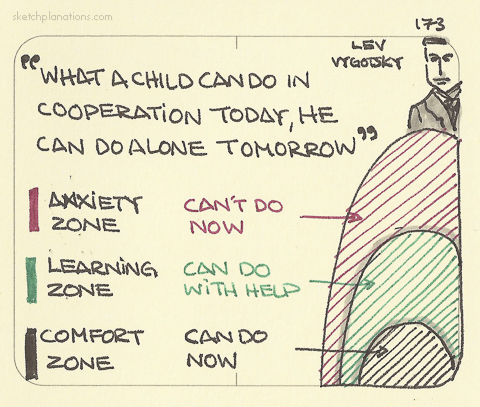
\includegraphics[width=13cm]{./images/zpd} \caption{A graphic interpretation of the Zone of Proximal Development}\label{fig:zpd}
\end{figure}

\subsection{Cognitivism}\label{cognitivism}

Contrary to the behaviourists, cognitivists argued that observable behaviors (see \ref{behaviorism}) are not sufficient to describe learning because the internal thought processes are also part of learning. On top of that, cognitivists posit that one can tell what happens in the human brain!
observable behaviors are not sufficient to describe learning because the internal thought processes are also part of learning.

In short, cognitivism is a learning theory that focuses on how information is received, organized, stored and retrieved by the mind. It uses the mind as an information processor. Or else, the human brain can be represented as a computer. Learners are actively involved in the way they process information. If we wants to improve and promote learning, then we should focus on developing knowledge, memory, thinking, and problem solving skills. Knowledge is viewed as symbolic mental constructs, or \textbf{schemata} (or else, representations). When learners' schemata change, learning takes place.

One of the most prominent representations of the human brain as a computer is portrayed in the Multi-store Model \citep{atkinson1968human} (see Figure \ref{fig:multistoremodel}). According to this model, human memory consists of three separate memory stores connected a linear sequence: the sensory memory, the short-term memory and the long-term memory. Learning happens as information is transferred between these stores, from the human sensors (for example, eyes and ears) until it is successfully stored in the long term memory.

\begin{figure}

\includegraphics[width=10cm]{./images/multistoremodel} \caption{A simplified representation of human memory according to the Multi-store Model}\label{fig:multistoremodel}
\end{figure}

Regarding the capacity of human memory, Sweller \citep{sweller1994cognitive} discussed the Cognitive Load Theory and explained how limitations of human memory can have a negative impact on learning. Specifically, Sweller argued that our working memory can hold a small amount of information at one time. Therefore, teaching should aim at avoiding overloading working memory if we want to support learning.

\href{https://en.wikipedia.org/wiki/John_Robert_Anderson_(psychologist)}{John Andrerson}, a Canadian-born and US-based psychologist, delivered one of the most well-known cognitive architecture (theory and computational instantiation of the structure of the human mind), ACT-R, that is used today by many modern Intelligent Tutoring Systems \citep{anderson2013architecture}. The key point that we keep from ACT-R is that human memory can be mapped into two parts:

\begin{itemize}
\tightlist
\item
  Declarative Memory: Here, humans store factual information, for example Paris is the capital of France.
\item
  Procedural Memory: Here, humans store information about procedures (What do I need to do to turn on the light?)
\end{itemize}

In 1997, Richard Mayer set the foundations of the Cognitive Theory of Multimedia Learning \citep{mayer1997multimedia}. Meyer defines multimedia as the presentation of material using both words and pictures. Thus, the definition of multimedia is narrowed down to two forms of information: verbal and visual. Mayer's theory is based on three assumptions (Mayer 2009):\\
1. Visual and auditory experiences or information are processed through separate and distinct information processing `channels'.\\
2. Each information processing channel is limited in its ability to process experiences or information.\\
3. Processing experiences or information in the channels form an active process designed to construct coherent mental representations.

In other words, people learn better when content is limited to the combination words + pictures. Combinations of pictures, words, sounds should be excluded. Also, people learn better when content is limited to combinations of narration + graphics rather than animation + text. Finally, graphics and narration work better than graphics + narration + text.

\section{Educational technology and educational technologies}\label{educational-technology-and-educational-technologies}

A lot of discussion has been going on lately about educational technology, and educational (or, learning) technologies. \textbf{Educational technology} is the research field that studies learners, their materials, tools and their environment.
\textbf{Educational technologies} are the tools we use to facilitate learning. Educational technologies don't have to be cutting edge. A pencil, a piece of paper or a projector can be considered as educational technologies.

Technology can be classified in two dimensions: Time and Space (Same Time/Space, Different Time/Space). The two dimensions refer to the physical presence of the learner and the instructor. For example, if the learner is at their home in Greece and the instructor is at their home in Germany but they both participate in the lecture via zoom at the same time, this would be classified as Same Time/Different Space.
This classification (see also Figure \ref{fig:timespacematrix}) is known as \emph{time-space matrix} \citep{johansen1988groupware}

\begin{figure}
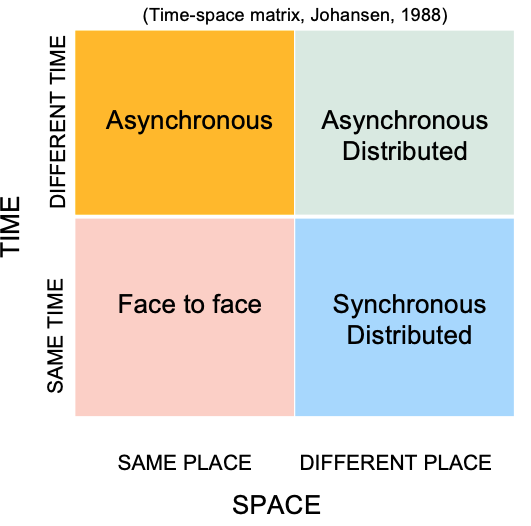
\includegraphics[width=13cm]{./images/time-space} \caption{The time-space classification matrix for Groupware Technologies according to Johansen[@johansen1988groupware]}\label{fig:timespacematrix}
\end{figure}

Another classification scheme that focuses on educational technologies is the Media Cube \citep{repenning1998learn}. The Media Cube classifies educational tools (or else, mediums) in three dimensions:

\begin{itemize}
\tightlist
\item
  Richness describes the degree to which elements from the real world are incorporated or represented within the medium.
\item
  Interactivity describes a continuum from passive observation to active exploration to active construction.
\item
  Accessibility describes how available the medium is and how easy it is not only to read what is created by others, but also to author new content.
\end{itemize}

\section{Educational Technologies and Learning Theories}\label{educational-technologies-and-learning-theories}

Learning Theories are reflected in the design and implementation of Educational Technologies. Here, we provide a few examples:

\begin{itemize}
\tightlist
\item
  Educational platforms that implement Game and Gamification elements, such as prizes and badges, are following the principles of Operand Conditioning (Behaviorism).
\item
  Similarly, classroom management tools that operate on the principle of positive and negative reinforcement.
\item
  Intelligent Tutoring Systems that adapt content and instruction based on a knowledge representation are designed on the principles of Cognitivism.
\item
  Learning Management Systems and tools for authoring learning content that present information in various formats(slides, videos, text) often follow the principles of the cognitive theory of multimedia learning.
\end{itemize}

\section{Intelligent Learning Environments}\label{intelligent-learning-environments}

The term ``Intelligent Learning Environents'' refers to learning environments (or else, educational technologies) that facilitate and promote human-centered learning, that is placing the learner at the center of the learning process. These aspects are demonstrated in the following definitions of Intelligent Learning Environments:
- ``\ldots a category of educational software in which the learner is `put' into a problem solving situation.'' \citep{dillenbourg1994intelligent}

\begin{itemize}
\tightlist
\item
  ``\ldots a learning environment that allows for student-driven learning'' \citep{kay1997learner}
\end{itemize}

Taking into account the above, Manolis Mavrikis and Wayne Holmes provided the following overarching definition for modern, intelligent learning environments:
``\emph{{[}intelligent learning environments is{]} a broad category of digital educational interactive applications equipped with features that enable the provision of personalized, adaptive support to students}'' \citep{mavrikis2019intelligent}

\section{Questions for Chapter \ref{learningtheories}}\label{questions-for-chapter-reflearningtheories}

\begin{enumerate}
\def\labelenumi{\arabic{enumi}.}
\tightlist
\item
  The quadratic model of time and space is a popular classification scheme for categorizing educational technology. Please describe and explain the model and provide examples for the four areas of the quadrant.
\item
  What is the difference between behaviorism and cognitivism?
\item
  Please explain the difference between constructivism and social constructivism.
\item
  Name a learning theory that is fundamental for designing intelligent learning environments. Give examples
\item
  How can we define ``Intelligent Learning Environments''?
\end{enumerate}

\section{To-Read}\label{to-read}

\begin{enumerate}
\def\labelenumi{\arabic{enumi}.}
\tightlist
\item
  \href{https://eddl.tru.ca/wp-content/uploads/2021/02/McLeod_from-learningmatters02durh.pdf}{McLeod, G. (2003). Learning theory and instructional design. learning matters, 2(3), 35-43.}
\end{enumerate}

\chapter{Intelligent Tutoring Systems}\label{its}

In 1920s, \href{https://en.wikipedia.org/wiki/Sidney_L._Pressey}{Sydney Pressey}, a psycology professor from Ohio State University, developed a mechanical artifact (that is, a \textbf{machine}) to provide standardized exercises to students for practicing. Pressey believed that `\textbf{the procedure in mastery of drill and informational material were in many instances simple and definite enough to permit handling of much routine teaching by mechanical means.}' Today, Pressey's `teaching machine' can be considered as the first attempt for designing Intelligent Tutoring Systems because not only it allowed students to practice on their own without the support of a teacher, but also because it provided real time feedback: Pressey fixed the machine so that the question remained until the student selected the correct answer.

Pressey's teaching machine encaptulates the premise of Intelligent Tytoring Systems (ITSs): allowing learners to practice on their own while they receive real-time feedback that addresses their individual needs. This premise is reflected in the following definition of ITSs: ``{[}an ITS is{]} a computer system that aims to provide immediate and customized instruction or feedback to learners.'' \citep{psotka1988intelligent} It is important to note that ITSs do not aim to replace the human tutor but, instead, to support humans in tutoring, enabling and facilitating their pracice.

\section{A brief history of Intelligent Tutoring Systems}\label{a-brief-history-of-intelligent-tutoring-systems}

One of -if not- the first intelligent tutoring program, SCHOLAR \citep{carbonell1970mixed} aimed at engaging learners in learning about georgaphy following a dialogue-based approach. That is, the ITS would ask and answer questions while keeping track of the ongoing dialogue structure. To do so, SCHOLAR was using in the background a semantic network to represent domain knowledge. In this way, the ITS could provide appropriate feedback to the learner, and at the same time, keep track of the knowledge that the learner was acquiring. However, computational limitations in sustaining a natural dialogue and complexity of designing and maintaining the domain knowledge representation made it challenging to develop and deploy such tutoring systems.

Following, coached practice became popular with ITSs like the PAT Algebra Tutor \citep{anderson1995cognitive}. In such environments, instruction is delivered as learners engage in problem solving tasks. Coached practice embodies the ``learning-by-doing'' model of cognitive skill acquisition: that is, learners are demonstrated how they should approach and deal with problem-solving and are asked to repeat this practice until they have mastered the skill at hand. As one may expect, problem-solving ITSs focus on STEM domains because of these domain's standardized formalism. Furthermore, a problem solving task constrains the solution and reasoning space for both the learner and tutor, because there is a finite number of acceptable solution. Therefore, the tutor can most of the times interpret the learner's action or - in worst case - offer some advice. This consequently means that coached practice with problem-solving tutors lowers the complexity that dialogue-based tutors face and are, therefore, easier to develop and deploy.

\section{Cognitive Tutors}\label{cognitive-tutors}

A sub-category of problem-solving ITSs are the Cognitive Tutors, that are based on ACT-R theory of skill knowledge \citep{anderson2013architecture}. This theory assumes a fundamental distinction between declarative knowledge and procedural knowledge (see \ref{learningtheories}). ACT-R assumes that skill knowledge is encoded initially in declarative form as informed by the learner's experience. Then, through practicing, the learner learns or constructs general rules while solving problems. These rules are encoded as procedural knowledge. For representing procedural knowledge, ACT-R uses production rules. These rules aim to describe the relationship between problem solving goals, learners' actions and states.

Remember the example we discussed in the class: how does a student learn to solve equations? Then looking at the interface of a math tutor (see Figure \ref{fig:mathtutor}), try to explain the problem-solving practice of a student and how the ITS captures the declarative and procedural knowledge.

\begin{figure}
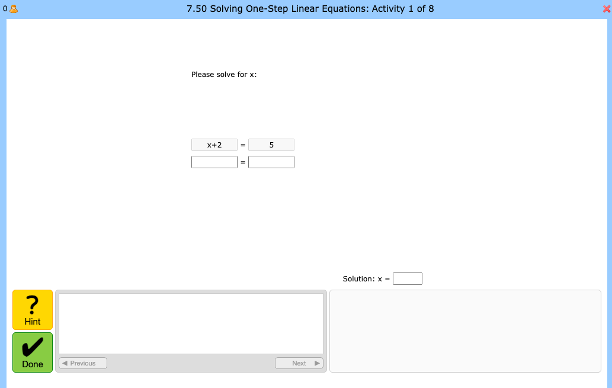
\includegraphics[width=13cm]{./images/mathtutor} \caption{An example interface of a math tutor, taken from the [CMU Math Tutors](https://mathtutor.web.cmu.edu/home)}\label{fig:mathtutor}
\end{figure}

\subsection{Model-tracing Tutors}\label{model-tracing-tutors}

Model-tracing tutors check learners' activity on the \emph{action} level. This means that they keep track of every action a learner makes while solving a problem, like for example ckicking a button. These tutors solve a problem concurrently with the learner and compare the learners' actions to an internal representation of the solution space (possible solutions). To represent the solution space, the model-tracing tutor uses sets of \textbf{production rules}. Then, depending on the result of this commparison, if the student action matches a production rule action it is assumed that the student has fired the same cognitive rule and the actions are carried out. If not, the tutor reports that it does not recognize the student's action.
The complete set of production rules that represent the solution space comprise the cognitive model.

\subsection{Example-tracing Tutors}\label{example-tracing-tutors}

In contrast to model-tracing tutors, the example-tracing tutors try to understand learners' behavior based on specific or typical examples of problem-solving behaviour. That is, instead of matching each action that the learners' can make to the solution space represented by production rules, they try to match the solution path of a learner to potential solutions. To provide real-time feedback, example-tracing tutors use behavior graphs. These graphs represent a finite number of typical solution paths a learner can follow when solving a problem.

\subsection{Knowledge-tracing Tutors}\label{knowledge-tracing-tutors}

Knowledge-tracing tutors are similar to model-tracing tutors. However, instead of tracing the learners' actions, they are used to calculate the required skills (\textbf{knowledge}) students learned. This can be done by employing knowledge graphs or bayesian knowledge models that assess learners' knowledge on specific knowedge components.

\section{Architecture of Intelligent Tutoring Systems}\label{architecture-of-intelligent-tutoring-systems}

The fundamental architecture of an ITS consists of four components (see Figure \ref{fig:itsarchitecture}):

\begin{itemize}
\tightlist
\item
  The interface component supports student interaction (input/output) with the ITS.
\item
  The domain model contains the rules, concepts, and knowledge related to the domain that should be learned.
\item
  The student model keeps track of the students' knowledge: their cognitive and affective states, and their progress as they learn. One may describe the student model as an annotated version of the domain model with information about the student's performance.
\item
  The pedagogical model uses the data gained from the domain model and student model to make decisions about instructional strategies such as when to give feedback, what kind of learning activity should be provided next to the student and if the student has mastered a skill and is ready to move to the next topic.
\end{itemize}

\begin{figure}
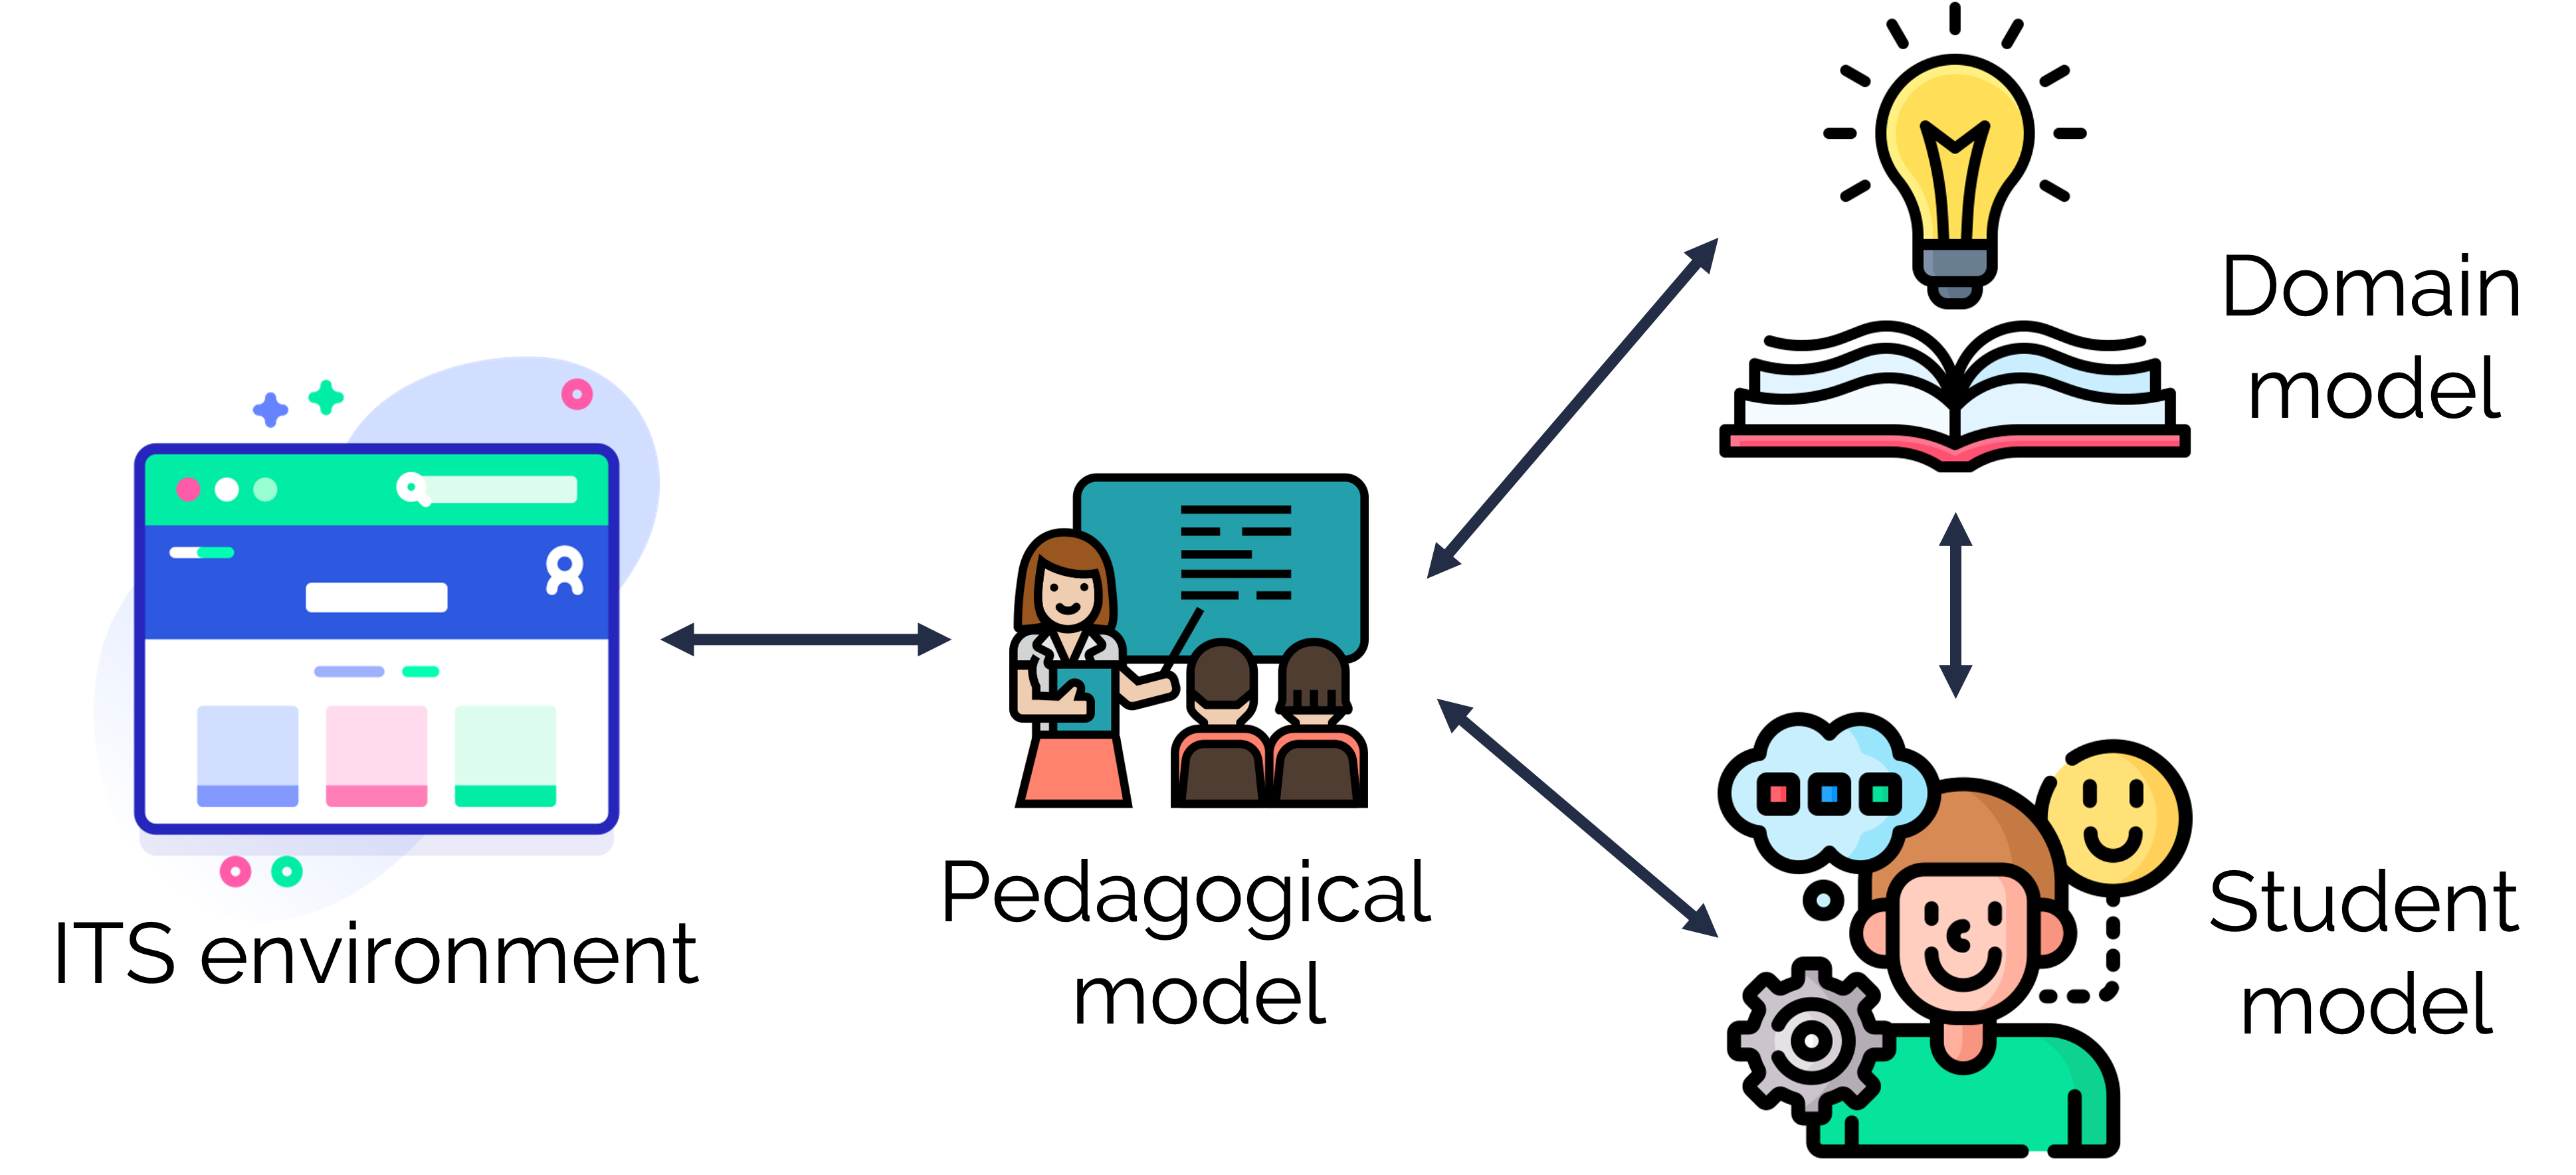
\includegraphics[width=13cm]{./images/ITSarchitecture} \caption{The architecture of an Intelligent Tutoring System}\label{fig:itsarchitecture}
\end{figure}

\section{Effectiveness of Intelligent Tutoring Systems}\label{effectiveness-of-intelligent-tutoring-systems}

In 1984, \href{https://en.wikipedia.org/wiki/Benjamin_Bloom}{Bejnamin Bloom} discussed the effectiveness of human tutoring. In his work, Bloom used the term ``human tutoring'' to refer to an adult, subject-matter expert working synchronously with a single student and suggested that human tutoring was the most effective kind of instruction, with an effect size of d = 2.0 relative to classroom teaching without tutoring \citep{bloom19842}. In contrast, CAI tends to produce an effect size of d = 0.31 \citep{kulik1991effectiveness}.

In 2011, Kurt VanLehn \citep{vanlehn2011relative} published a wide review of ITS-related studies that demonstrated the following:
1. human tutoring is not as effective as we once thought;
2. ITS are almost as effective as adult, one-on-one human tutoring;
3. None of the studies replaced a classroom teacher with ITS.

Based on the above, Van Lehn concluded that ITSs are indeed as effective as human tutors in the condition where ITSs are used along classroom instruction. Thus, ITSs could be used to replace homework in order to enhance practice outside the classroom, but not as a substitute of the classroom experience.

\section{Questions for Chapter \ref{its}}\label{questions-for-chapter-refits}

\begin{enumerate}
\def\labelenumi{\arabic{enumi}.}
\tightlist
\item
  What is an intelligent tutoring system? Definition, principles, and basic architecture.
\item
  What is / are the fundamental learning theory or theories behind Intelligent Tutoring Systems? Please elaborate.
\item
  What is the basic architecture of Intelligent Tutoring Systems and what are their fundamental components?
\item
  There is a saying that human tutoring is the golden standard. What do you think?
\item
  What is the difference between model-tracing, example-tracing and knowledge-tracing ITSs?
\item
  What are the behavior graphs that are typically used by example-tracing tutors?
\end{enumerate}

\section{To-Read}\label{to-read-1}

\begin{enumerate}
\def\labelenumi{\arabic{enumi}.}
\tightlist
\item
  \href{http://act-r.psy.cmu.edu/wordpress/wp-content/uploads/2012/12/173Chapter_37_Intelligent_Tutoring_Systems.pdf}{Corbett, A. T., Koedinger, K. R., \& Anderson, J. R. (1997). Intelligent tutoring systems. In Handbook of human-computer interaction (pp.~849-874). North-Holland.}
\item
  \href{https://scholar.google.com/scholar?hl=en&as_sdt=0\%2C5&scioq=Toward+combining+individual+and+collaborative+learning+within+an+intelligent+tutoring+system.+In\%C2\%A0Artificial+Intelligence+in+Education&q=Example-Tracing+Tutors\%3A+A+New+Paradigm+for+Intelligent+Tutoring+Systems&btnG=\#:~:text=include\%20citations-,\%5BPDF\%5D\%20cmu.edu,-\%5BPDF\%5D\%20Example}{Aleven, V., McLaren, B., Sewall, J., \& Koedinger, K. R. (2009). Example-tracing tutors: A new paradigm for intelligent tutoring systems.}
\end{enumerate}

\chapter{Student Modeling}\label{studentmodels}

Going back to the definition of Intelligent Learning Environments (see Chapter \ref{learningtheories}) and Intelligent Tutoring Systems (see Chapter \ref{its}), it is evident that in order to provide personalized support tailored to the learners' individual needs, one needs to maintain an accurate and up-to-date representation of individual students. And, one may ask: ``\emph{How?}''

When discussing about the architecture of Intelligent Tutoring Systems (Chapter \ref{its}), we talked about a fundamental compontent: \textbf{the student model} and we described it as containing knowledge about the students: their cognitive and affective states, and their progress as they learn. Peter Brusilovsky provided the following definition for student models:

``\emph{A student model is a representation within the architecture of an intelligent learning environment (ILE) of a student's understanding of material being taught}'' \citep{brusilovsky1994student}

\section{Learning Curve and Predicted Learning Curve}\label{learning-curve-and-predicted-learning-curve}

An old saying states that ``practice makes better'' and another one says that ``repetition is the mother of learning''. From our own experience, we can attest that learning happens as humans practice over time. This idea is depicted by the concept of the Learning Curve (see Figure \ref{fig:learningcurve}). Practically, this curve shows that the more a human practices a skill or a piece of knowledge, the more they learn.

\begin{figure}
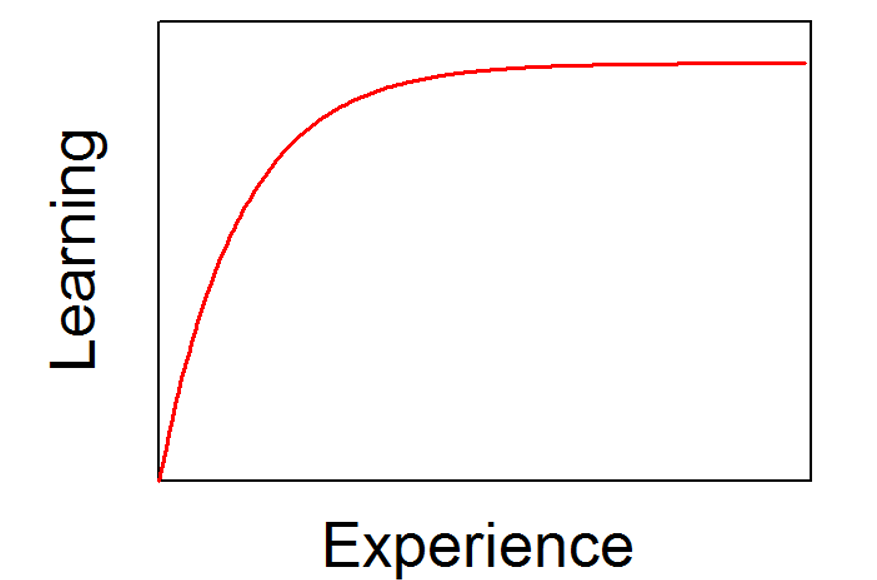
\includegraphics[width=10cm]{./images/learningcurve} \caption{An ideal learning curve that demonstrates the relationship between experience and learning}\label{fig:learningcurve}
\end{figure}

Figure \ref{fig:learningcurve} shows an ideal curve and Figure \ref{fig:learningcurvestages} shows different stages of the learning process, as they can be traced on a learning curve.

\begin{figure}
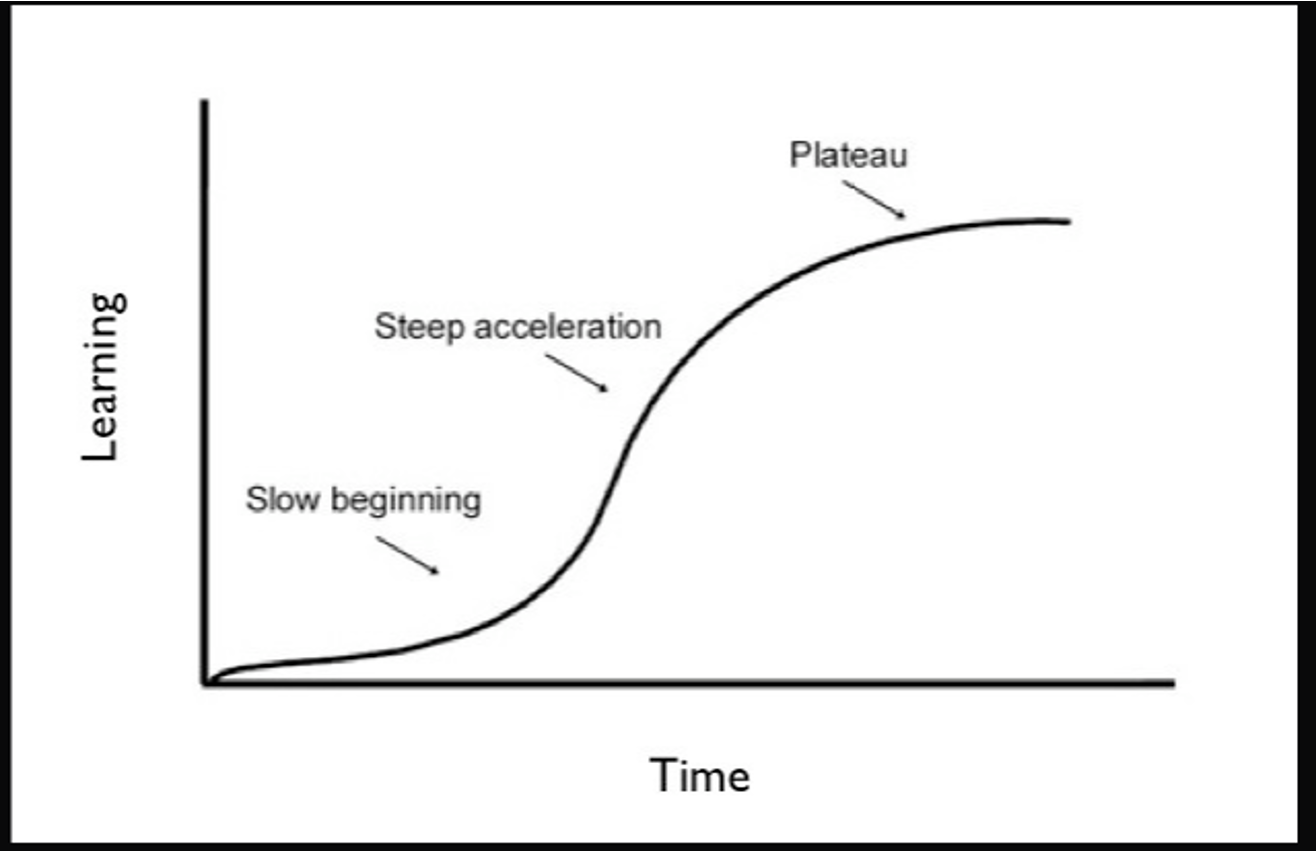
\includegraphics[width=10cm]{./images/learningcurvestages} \caption{The different stages of the learning process as depicted on an ideal learning curve that demonstrates the relationship between time and learning}\label{fig:learningcurvestages}
\end{figure}

In reality, an empirical learning curve (that is, the average correct responses for a skill over each learning opportunity) as calculated by data is not as smooth as the ideal learning curve (see Figure \ref{fig:empiricallearningcurve}. This may happen due to recording errors, but also to the complicated nature of learning (such as forgetting or slipping).

\begin{figure}
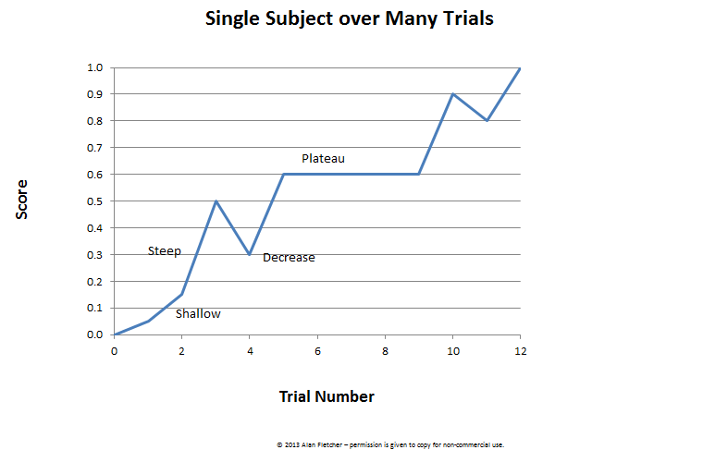
\includegraphics[width=10cm]{./images/empiricallearningcurve} \caption{The different stages of the learning process as depicted on a more realistic learning curve}\label{fig:empiricallearningcurve}
\end{figure}

To operationalize mastery learning and learning curves in the context of student models and intelligent tutoring systems, the predicted learning curve is used instead since it is easier to calucate but also much smoother. To compute the predicted learning curve, typically an item-response theory (IRT) model is used (either the Additive Factor Model (AFM) or one of the same family). This model predicts how a student will perform for each skill on each learning opportunity. The predicted learning curve practically shows the average predicted error of a skill (y-axis) over each of the learning opportunities (x-axis) (see Figure \ref{fig:predictedlearningcurve}).

Precicted learning curves may reveal the following \citep{cen2007over}:
1. How much practice a student needs to master a skill; Ideally, a predicted learning curve should start high and end high (why?)
2. What is the optimal set of skills to match the learners' needs; as before, a predicted learning curve should start high and end high (why?)

\begin{figure}
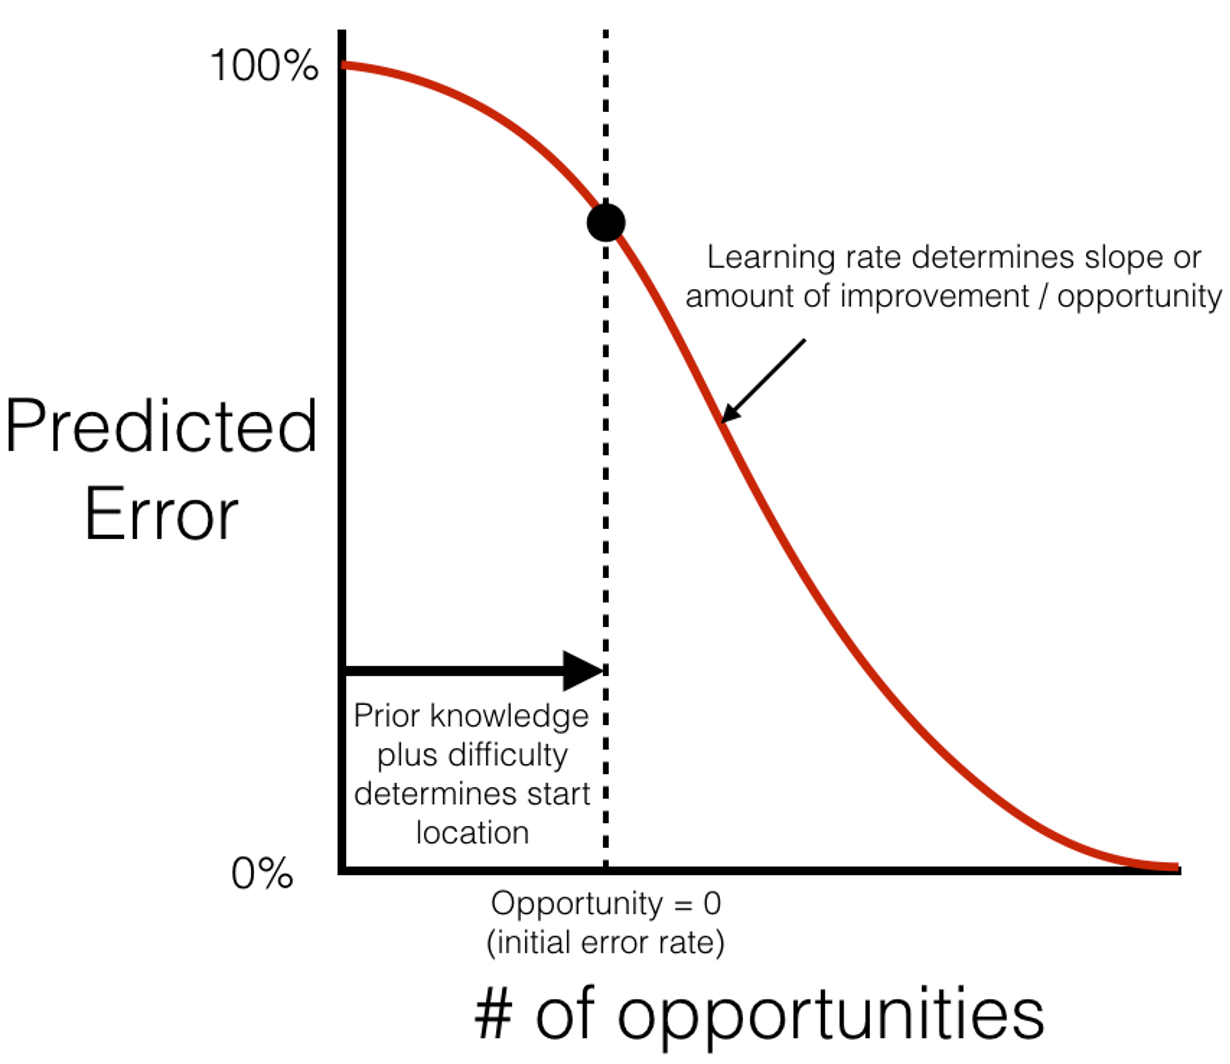
\includegraphics[width=10cm]{./images/predictedlearningcurve} \caption{The predicted learning curve shows a precise prediction of students' success rate at each learning opportunity}\label{fig:predictedlearningcurve}
\end{figure}

\section{Overlay Student Models}\label{overlay-student-models}

Student models that track student's knowledge as subset of the expert/system's knowledge of domain (domain model) are called Overlay Student Models. These models may be \emph{perceived} annotated versions of the knowledge representations used by domain models that asssess learners' knowledge. Overlay student models track some pedagogically relevant measurement as a function of the overlay type (for example, skills, facts, or concepts). Here we will discuss two kinds of overlay models: item-response theory models and model-tracing models \citep{pavlik2013tutoring}.

\subsection{Item-Response Theory Models}\label{item-response-theory-models}

The Item-Response Theory (IRT) (or else, latent response theory) premise is to calculate the probability of a correct response to an item as a mathematical function of person and item parameters. In practice IRT aims to explain the relationship between latent traits (unobservable characteristics or attributes) and their manifestations (observed outcomes, responses or performance). To do so, one should establish a link between the properties of items on an instrument (this can be a knowledge questionnaire), learners' responding to the items of the questionnaire and the underlying trait being measured (that is, learning). IRT models typically use a structure called Q-matrix to represent the relationship between instrument items' and learners' responses.

Three typical IRT models are the Additive Factors Model (AFM), the Performance Factors Model (PFM) and the Instructional Factors Model (IFM). Briefly:

\begin{itemize}
\tightlist
\item
  the Additive Factor Models (AFM): Use logistic regression to predict the probability that the student answers a question/item correctly. To make this prediction, the AFM uses the student's prior knowledge, the difficulty of the item, the learning rate of the student (that is, how fast the student learns) and the number of practicing opportunities \citep{cen2006learning};
\item
  the Performance Factor Models (PFM): Same as the AFM but it differentiates opportunities based on correct and incorrect responses. That is, the prediction is made depending on student's prior knowledge, difficulty of the item, learning rate of the student and the number of correct and incorrect prior opportunities \citep{pavlik2009performance};
\item
  the Instructional Factor Models (IFM): Same as the PFM but this time the model takes into account the ``tells''. that is, how many times the tutor gave the student the correct answer or additional help \citep{chi2011instructional}.
\end{itemize}

\subsection{Model-tracing Models}\label{model-tracing-models}

Model-tracing models operational principle is to encode the domain model (expert solution) as a set of production rules and compare the student's actions to the domain model. In this way, the tutor tries to understand student actions. If the student's action is the same as the domain model, then everything is great! If the student's action match to some extent then the tutor will follow up with alternative questions to ensure learning. If the student's action does not match with the domain model, then the tutor is not able to understand the error. The tutor will continue asking the question until the student's response matches to the domain model.

One of the most well-know modeling approaches for implementing model-tracing models is Bayesian Knowledge Tracing (BKT). BKT is typically used to track students' progress from one problem to the next relative to production rules practically mapping students' skills either as learned or unlearned. BKT predicts whether a student has learned a skill based on four probabilities \citep{corbett1994knowledge}:

\begin{itemize}
\tightlist
\item
  P(known):~the probability that the student already knew a skill.
\item
  P(will learn):~the probability that the student will learn a skill on the next practice opportunity.
\item
  P(slip):~the probability that the student will answer incorrectly despite knowing a skill.
\item
  P(guess):~the probability that the student will answer correctly despite not knowing a skill.
\end{itemize}

\section{Questions for Chapter \ref{studentmodels}}\label{questions-for-chapter-refstudentmodels}

\begin{enumerate}
\def\labelenumi{\arabic{enumi}.}
\tightlist
\item
  ``Student models'': Provide a definition, purpose, and examples.
\item
  What are the basic modeling parameters for Bayesian Knowledge Tracing (BKT)?
\item
  What is Item Reponse Theoty and what are the Item Response Theory (IRT) models?
\item
  What is the relationship between student models and the learning curve?
\item
  How is the learning curve operationalized in Intelligent Tutoring Systems?
\item
  A family of common student models is the Item Response Theory (IRT) models and in particular, the AFM, the PFM, and the IFM. Explain what are the similarities and differences between these models, how can they be implemented (regression functions) and relate your response to theories of cognition and learning. Please elaborate on how the models' differences may impact their performance in terms of accuracy and goodness of fit.
\end{enumerate}

\section{To-Read}\label{to-read-2}

\begin{enumerate}
\def\labelenumi{\arabic{enumi}.}
\tightlist
\item
  \href{https://citeseerx.ist.psu.edu/document?repid=rep1&type=pdf&doi=040d21fb726c5175eca9e37801031519f06e0d86\#page=63}{Pavlik Jr, P. I., Brawner, K., Olney, A., \& Mitrovic, A. (2013). Tutoring systems. Des. Recommendations Intell. Tutoring Syst, 1, 39-68.}
\item
  \href{http://pact.cs.cmu.edu/pubs/Cen\%2C\%20Koedinger\%20\%26\%20Junker06.pdf}{Cen, H., Koedinger, K., \& Junker, B. (2006, June). Learning factors analysis--a general method for cognitive model evaluation and improvement. In International conference on intelligent tutoring systems (pp.~164-175). Berlin, Heidelberg: Springer Berlin Heidelberg.}
\item
  \href{http://pact.cs.cmu.edu/pubs/AIED\%202009\%20final\%20Pavlik\%20Cen\%20Keodinger\%20corrected.pdf}{Pavlik, P. I., Cen, H., \& Koedinger, K. R. (2009). Performance factors analysis--a new alternative to knowledge tracing. In Artificial intelligence in education (pp.~531-538). Ios Press.}
\item
  \href{http://pact.cs.cmu.edu/pubs/Chi,\%20Koedinger\%20Gordon,\%20Jordon\%20&\%20VanLehn\%20-\%20edm2011.pdf}{Chi, M., Koedinger, K. R., Gordon, G. J., Jordon, P., \& VanLahn, K. (2011). Instructional factors analysis: A cognitive model for multiple instructional interventions.}
\item
  \href{http://act-r.psy.cmu.edu/wordpress/wp-content/uploads/2012/12/893CorbettAnderson1995.pdf}{Corbett, A. T., \& Anderson, J. R. (1994). Knowledge tracing: Modeling the acquisition of procedural knowledge. User modeling and user-adapted interaction, 4, 253-278.}
\end{enumerate}

\chapter{Collaborative Learning}\label{cits}

As we saw in earlier chapters, bevaviorism and cognitivism put emphasis on the individual when trying to decode and explain how learning happens. In contrast, social constructivism explores learning in a social environment and perceives the learner and other roles in their environment as a system.

Collaborative learning builds on the premise of social constructivism. In particular, collaborative learning can be described as ``\emph{a situation in which two or more people learn or attempt to learn something together}''\citep{dillenbourg1999you}. Collaborative learning is considered critical because it allows learners to learn and practice not only knowledge relating to a specific domain (such as physics or mathematics) but also social and soft skills, much needed for navigating within a social context. In particular, research has established that collaborative learning supports practicing communication and critical thinking skills, it is beneficial for learners' confidence and it fosters enjoyement. Also, it promotes diversity and building trust while improving creativity and encouraging commitment.

The practice of using computers as a means to mediate collaborative learning situations is called Computer-Supported Collabroative Learning (CSCL). In other words, CSCL is ``\emph{a pedagogical approach wherein learning takes place via social interaction using a computer or through the Internet}''\citep{stahl2006cambridge}

\section{Computer-Supported Collaborative Learning Environments}\label{computer-supported-collaborative-learning-environments}

CSCL Learning Environments allow learners to interact with each other and carry out learning activities in collaboration. Such environments typically offer a common workspace where learners can co-create diagrammatic representations like algorithmic flowcharts or concept maps and some additional tool to facilitate communication, for example a chat tool (see Figure \ref{fig:synergo}.

\begin{figure}
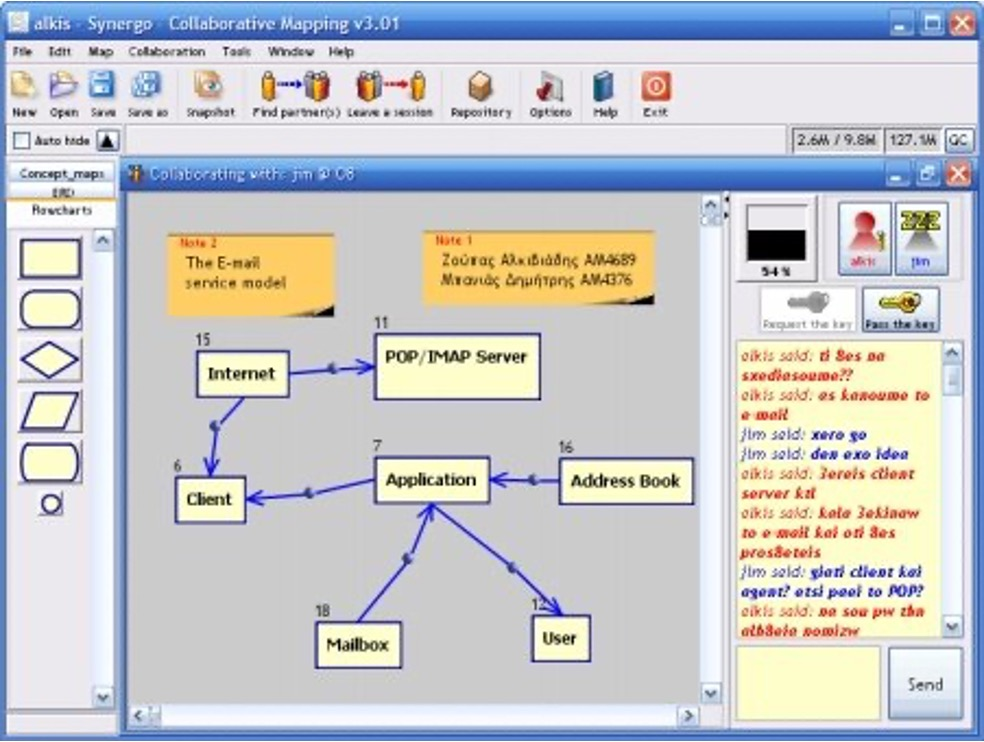
\includegraphics[width=13cm]{./images/synergo} \caption{Synergo, a CSCL tool to support students who learned introduction to programming}\label{fig:synergo}
\end{figure}

Most CSCL environments fall into one of the following three categories \citep{soller2005mirroring}:

\begin{itemize}
\tightlist
\item
  Mirroring: these are tools that automatically collect and process data regarding the learners' interaction. Then, they present this information to the learners (usually through visualizations) in order to raise learners' awareness and support self-reflection.
\item
  Monitoring: such tools provide information about what the ideal collaboration and interaction should look like and compare this ideal state with the current practice. Monitoring tools aim to support learners but also teachers in diagnosing problems that the learners may encounter.\\
\item
  Guiding: these tools include all functions that mirroring and monitoring tools perform and additionally, they propose remedial actions to help the learners.
\end{itemize}

\section{Collaborative Intelligent Tutoring Systems (CITSs)}\label{collaborative-intelligent-tutoring-systems-citss}

Intelligent Tutoring Systems (ITSs) have been criticized for their focus on individual learning and for the lack of support for social aspects of learning. To address this criticism, research has lately explored the use of ITSs for supporting collaborative learning. Such systems, named Collaborative Intelligent Tutoring Systems (CITSs), are
``\emph{learning systems that integrate Artificial intelligence into
collaborative learning environments. CITSs have evolved from
both ITS and CSCL}.'' \citep{ubani2022review} Research in CITSs has focused on supporting peer tutoring and adaptive collaborative learning support (ACLS), problem-based learning and scripted collaboration.

\subsection{Adaptive Collaborative Learning Support}\label{adaptive-collaborative-learning-support}

CITSs that focus on adaptive collaborative learning support (ACLS) adapt their characteristics, and sometimes provide intelligent hints and feedback, to improve students' collaborative interactions. In such situations, learners typically engage in peer-tutoring scenarios where one learner plays the role of the ``student'' and the other learner plays the role of the ``teacher''. The CITS monitors both the activity of the ``student'' and the ``teacher'' and provides feedback or guidance either to one or both of them to support their practice.

An example of such a system is the Adaptive Peer Tutoring Assistant (APTA) \citep{walker2014adaptive} that aims to support students who learn algebra. Through the CITS, the learner who plays the role of the ``teacher'' can watch the ``student'' take problem-solving actions and then, the ``teacher'' can mark the actions as right or wrong. The learners can communicate using a chat tool and in the same way, they can receive prompts from the CITS, which in turn they can choose to like, dislike or simply ignore.

\subsection{CITSs for Problem-based Learning}\label{citss-for-problem-based-learning}

CITS for Problem-based learning focus on modeling individual knowledge and activity in similar ways like traditional ITSs do (for example,with the use of Bayesian networks) but engaging learners in collaborative activities on shared workspaces.
In such settings, the learners participate in group discussions that are guided by the system. In this way, learners can both use the help of hints provided by the system but also take advantage of discussions with peers.

\subsection{CITSs for scripted collaboration}\label{citss-for-scripted-collaboration}

Apart from CITSs that aim to support domain knowledge (such as, math or physics), some systems aim to support soft skills, such as collaboration and communication along with domain knowledge. To do so, these systems build upon established paradigms of ITSs and they add support targeting soft skills.
For example, \citep{olsen2016investigating} designed a CITS that used a basic ITS for fractions but integrated collaborative scripts to support collaboration. In particular, the collaborative scripts were used by the system in order to distribute tasks and responsibilities to the learners who worked in groups in a structured manner but also in order to provide hints that aimed to help them in collaboration.

\section{Questions for Chapter \ref{cits}}\label{questions-for-chapter-refcits}

\begin{enumerate}
\def\labelenumi{\arabic{enumi}.}
\tightlist
\item
  What is computer-supported collaborative learning and what is the learning theory that inspired this learning paradigm?
\item
  What are Collaborative Intelligent Tutoring Systems (CITS)? Explain how they function and how they support learning using one example.
\item
  What is the difference(s) between Intelligent Tutoring Systems and Collaborative Intelligent Tutoring Systems? When would you use an ITS, and when would you use a CITS?
\end{enumerate}

\section{To-Read}\label{to-read-3}

\begin{enumerate}
\def\labelenumi{\arabic{enumi}.}
\tightlist
\item
  \href{https://www.researchgate.net/publication/37452559_Basics_of_Computer-Supported_Collaborative_Learning}{Pierre, D., \& Frank, F. (2007). Basics of Computer-Supported Collaborative Learning. Zeitschrift für Berufs-und Wirtschaftspädagogik,(21), 111-130.}
\item
  \href{https://telearn.hal.science/file/index/docid/197378/filename/Soller-Amy-2005.pdf}{Soller, A., Martinez, A., Jermann, P., \& Muehlenbrock, M. (2005). From mirroring to guiding: A review of state of the art technology for supporting collaborative learning. International Journal of Artificial Intelligence in Education, 15(4), 261-290.}
\end{enumerate}

\chapter{Artificial Intelligence in Education}\label{aied}

\section{What is Intelligence?}\label{what-is-intelligence}

``Intelligence'' is a complex construct with no clear concise definition. Instead ``\emph{there seem to be almost as many definitions of intelligence as there were experts asked to define it.}'' \citep{legg2007collection}. However, going through various definitions from multiple disciplines and domains, make it evident that learning, sense-making and ability to adapt are integral parts of intelligence. Other attempts to define intelligence include the capacity to aquire and apply knowledge, the capacity to solve new problems the ability of a system to act appropriate in uncertain environments.

\section{What is Artificial Intelligence?}\label{what-is-artificial-intelligence}

Similarly to ``intelligence'', a unique definition of ``Artificial Intelligence'' (AI) is hard to be widely adopted.
John McCarthy, who has been attributed as coining the term Artificial Intelligence, describes AI as computational technologies that allow machines to act and take decisions imitating human behavior and intelligence: ``\emph{It is the science and engineering of making intelligent machines, especially intelligent computer programs. It is related to the similar task of using computers to understand human intelligence, but AI does not have to
confine itself to methods that are biologically observable.}'' \citep{mccarthy2007artificial}.

It is important to remember though, that we're talking about machine-based intelligence, where human-defined objectives are turned into predictions, recommedations or decisions. ``Intelligent'' machines \textbf{appear} to work autonomously and can adapt their function as they ``learn'' from the environment. These important points are demonstrated in the definition provided by \href{https://www.unicef.org/globalinsight/media/2356/file/UNICEF-Global-Insight-policy-guidance-AI-children-2.0-2021.pdf}{UNICEF} that defines AI as: ``\emph{AI refers to machine-based systems that can, given a set of human-defined objectives, make predictions, recommendations, or decisions that influence real or virtual environments. AI systems interact with us and act on our environment, either directly or indirectly. Often, they appear to operate autonomously, and can adapt their behaviour by learning about the context.}''

AI finds application in many fields, including among others government (military), manufacturing, media, law, , health care, internet platforms and \textbf{education}.

\section{Artificial Intelligence in Education (AIED)}\label{artificial-intelligence-in-education-aied}

Artificial Intelligence in education (AIED) is an academic field of enquiry, officially established in the 1980s, that primarily researches AI tools to support learning (i.e.~`learning with AI'). It does NOT include aspects of learning about AI or preparing to live with AI (AI Literacy).

\subsection{A Bit of History}\label{a-bit-of-history}

Although the field itself was established in the 80s, it has roots way earlier (see Figure \ref{fig:aiedstory}. For example, \href{https://en.wikipedia.org/wiki/Herbert_A._Simon}{Herbert Simon} and \href{https://en.wikipedia.org/wiki/Allen_Newell}{Allen Newell} wrote in the '50s a computer program, \textbf{the logical theorist} that could prove mathematical theorems and in some cases it produced the same or better results than actual mathematicians :) In the '70s, LOGO - a general purpose programming language - was used to teach students about geometry with the use of visualizations. In the 90's, John Anderson proposed the cognitive architecture ACT-R that set the foundations for modern Cognitive Tutors.

\begin{figure}
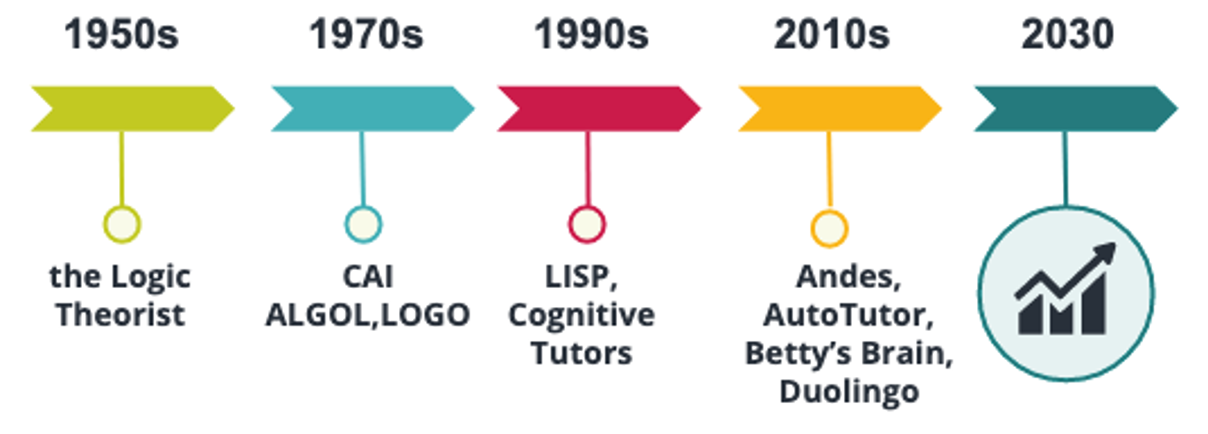
\includegraphics[width=10cm]{./images/AIEDhistory} \caption{A timeline of AIED}\label{fig:aiedstory}
\end{figure}

\subsection{AIED Premises}\label{aied-premises}

AIED is exploring the use of AI as a means to support teaching and learning. As such, it involves the use of AI-driven tools in teaching and learning, and includes:

\begin{itemize}
\tightlist
\item
  the use of AI to support learners directly (learner-supporting AI) AI involving tools such as Intelligent Tutoring Systems, chatbots, and AI to support learners with disabilities. It does not aim to replace teachers but to act supplementary.
\item
  the use of AI to support teachers directly (teacher-supporting AI) with tasks such as automatic assessment, and retrieving or smart curation of learning materials. Main applcation cases involve teacher-facing dashboards that display information about students, recommender systems that propose materials for teachers to be used in the classroom, tools for grading essays or reports and systems that help teachers with drafting lesson plans.
\item
  the use of AI to support education institutions (institution-supporting AI) with tasks such such as admissions, timetabling, communication and learning management.
\end{itemize}

\section{AI Methods in Education}\label{ai-methods-in-education}

Using AI to learn \emph{about} learners and learning is not strictly AI. However, there is an overlap when it involves the analysis of learning data or learning traces using computational algorithms. This overlapping but nonetheless distinct field is usually known as learning analytics or educational data mining. The methods most commonly used in this field of AIED can be grouped into three categories \citep{hoppe2017computational}:

\begin{itemize}
\tightlist
\item
  Content-oriented Methods: These methods aim to analyse learner-generated artifacts (such as reports, concept maps, assignments). Based on the analysis of such articats, we can understand how people learn.
\item
  Process-oriented Methods: These methods explore the processes that humans apply when learning as manifestated by their activity. For example, the sequence analysis of learners' activity in an LMS platform (e.g.~Moodle).
\item
  Network-based Methods: These methods aim to explore social aspects of learning, such as how learners explore with other roles, for example teachers or other learners, in the context of learning.
\end{itemize}

\section{FATE}\label{fate}

Computers, and AI are becoming fundamental parts of our everyday life, and the impact they have on society is considerable. Are algorithms objective, impartial, fair and accurate? Is AI Fair, Accountable, Trasparent and Ethical (FATE)?
We like data and choose things based on data, because they give us a sense of impartiality and subjectivity. We - as humans - do it either when computers are involved or not. However, one thing we cannot ignore, is that algorithms, and algorithms decision-making can be biased.

Bias can infiltrate in all stages of AI development and deployment including the data (imbalanced / biased data), the models (interpretability, performance), the training and deployment (feedback loops) and evaluation (lack of rigorous analysis, human errors).

\subsection{AI Bias}\label{ai-bias}

Two common types of AI-manifested biases are data-driven bias and interpretation-driven bias.
Interpretation-driven bias arises due to our false assumptions and errors about how the models' function or the interpretation of their results.
Data-driven bias arises due to problems in the data that we use to train AI. Three commonly occurring data-driven biases are: selection bias (when the data selection is not randomized), reporting bias (when what we communicate does not reflect the real likelihood, for example news coverage typically focusing on extreme cases) and sampling bias (when specific instances are sampled more frequently, for example sampling more chocolates rather than fruit). Such biases are driven by class or feature imbalances that are hidden in the data.

\subsubsection{Bias due to class imbalance}\label{bias-due-to-class-imbalance}

Class imbalance can occur when the real population distribution (see Figure \ref{fig:classdistribution}) does not match the sample population distribution (see Figure \ref{fig:classimbalance}) that is used to train the AI algorithm. This is a problem because the prediction always follows training. So if the model is trained on a sample that one class is the majority, then the prediction will favor the majority class.

\begin{figure}

\includegraphics[width=8cm]{./images/classdistribution} \caption{The real population distribution of beavers in the wild nature}\label{fig:classdistribution}
\end{figure}

\begin{figure}

\includegraphics[width=8cm]{./images/classimbalance} \caption{The sample population distribution of beavers used for AI training}\label{fig:classimbalance}
\end{figure}

To solve this problem, one should ensure that either the sample population reflects reality (batch selection) or, if this is not possible, to give more importance to the rare case (weighting).

\subsubsection{Hidden Bias}\label{hidden-bias}

Sometimes, there may be hidden features or attributes that affect the balance of the dataset but they are hard to account for, either because they are not explicitly related to the features one want to model or because they are simply not visible and not considered. However, these features can still come into play when training AI algorithms and lead to bias.
In the beavers' example (see Figure \ref{fig:classdistribution}), such an attribute could be the sex of the beavers that, when left unaccounted could lead to favoring male beavers over female beavers since, depending on the sampling, can end up being the majority class (see Figure \ref{fig:beavershidden}).

\begin{figure}
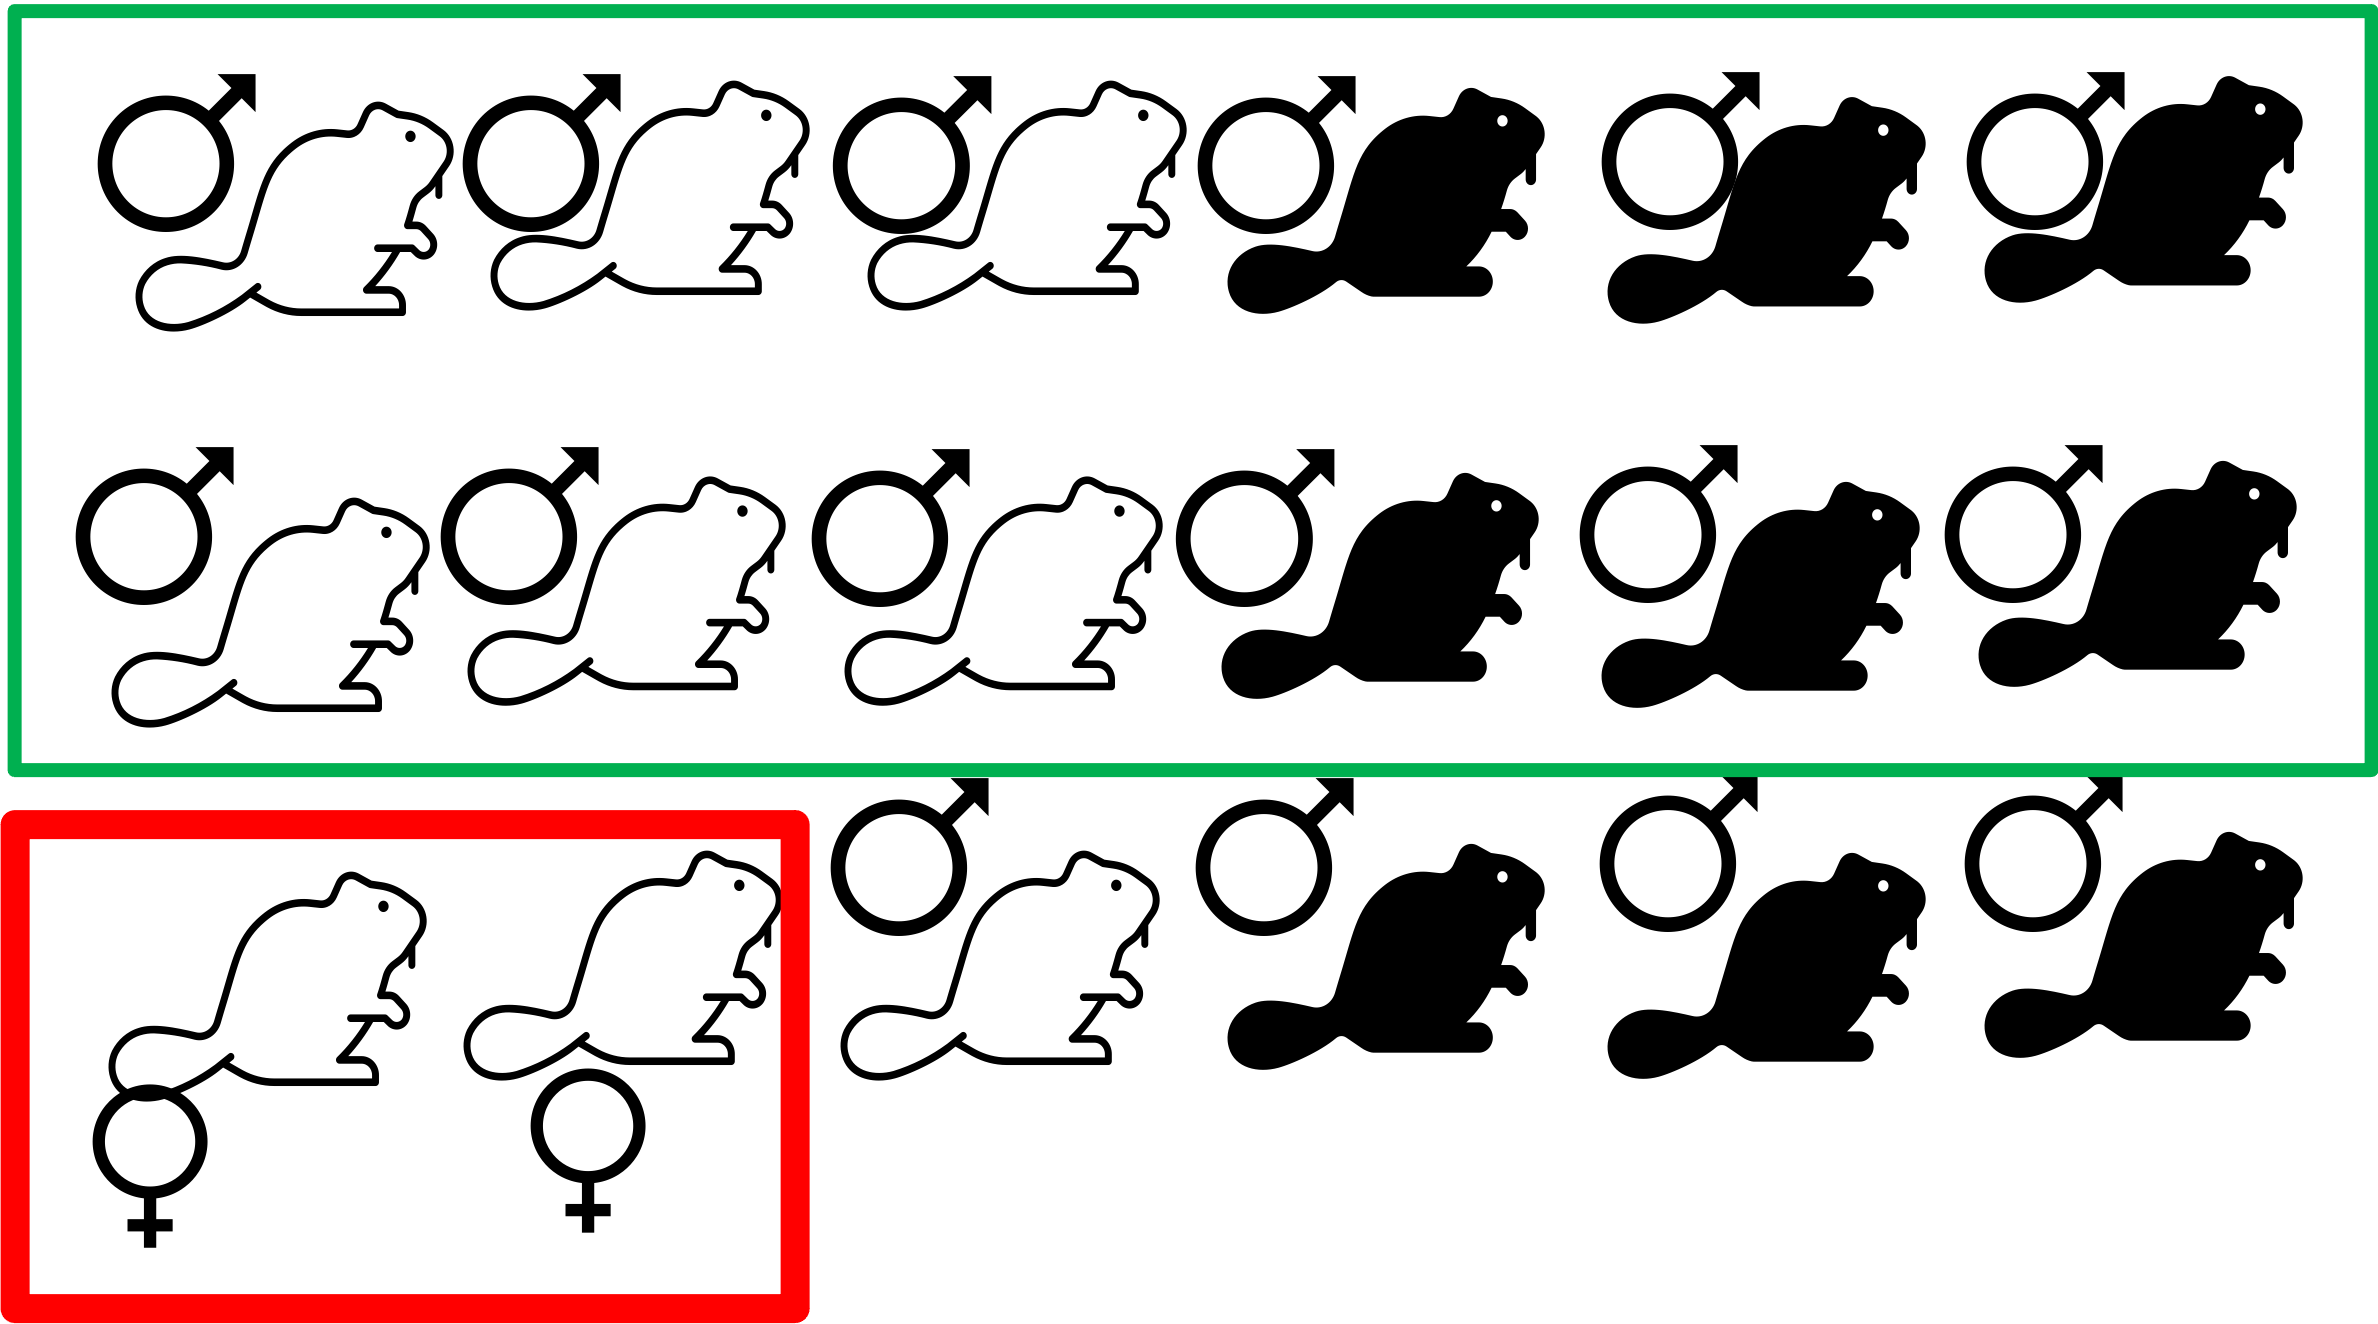
\includegraphics[width=10cm]{./images/beaverssex} \caption{The sample population distribution of beavers marked with the hidden feature}\label{fig:beavershidden}
\end{figure}

\subsubsection{Distribution Shift}\label{distribution-shift}

In some cases, we train our algorithms using curated datasets that does not completely align with the target population. For example, lets assume that we want to train an algorithm to predict whether an image shows a cat or a dog and we train the algorithm with pictures of real cats and dogs. Then we try to apply the algorithm on images that show sketches of cats and dogs instead of real animals (see Figure \ref{fig:catsanddogs}). This distribution shift (the model being trained on one manifestation of cats and dogs - real animals - and applied on another -sketches ) can lead to overgeneralization bias.

\begin{figure}
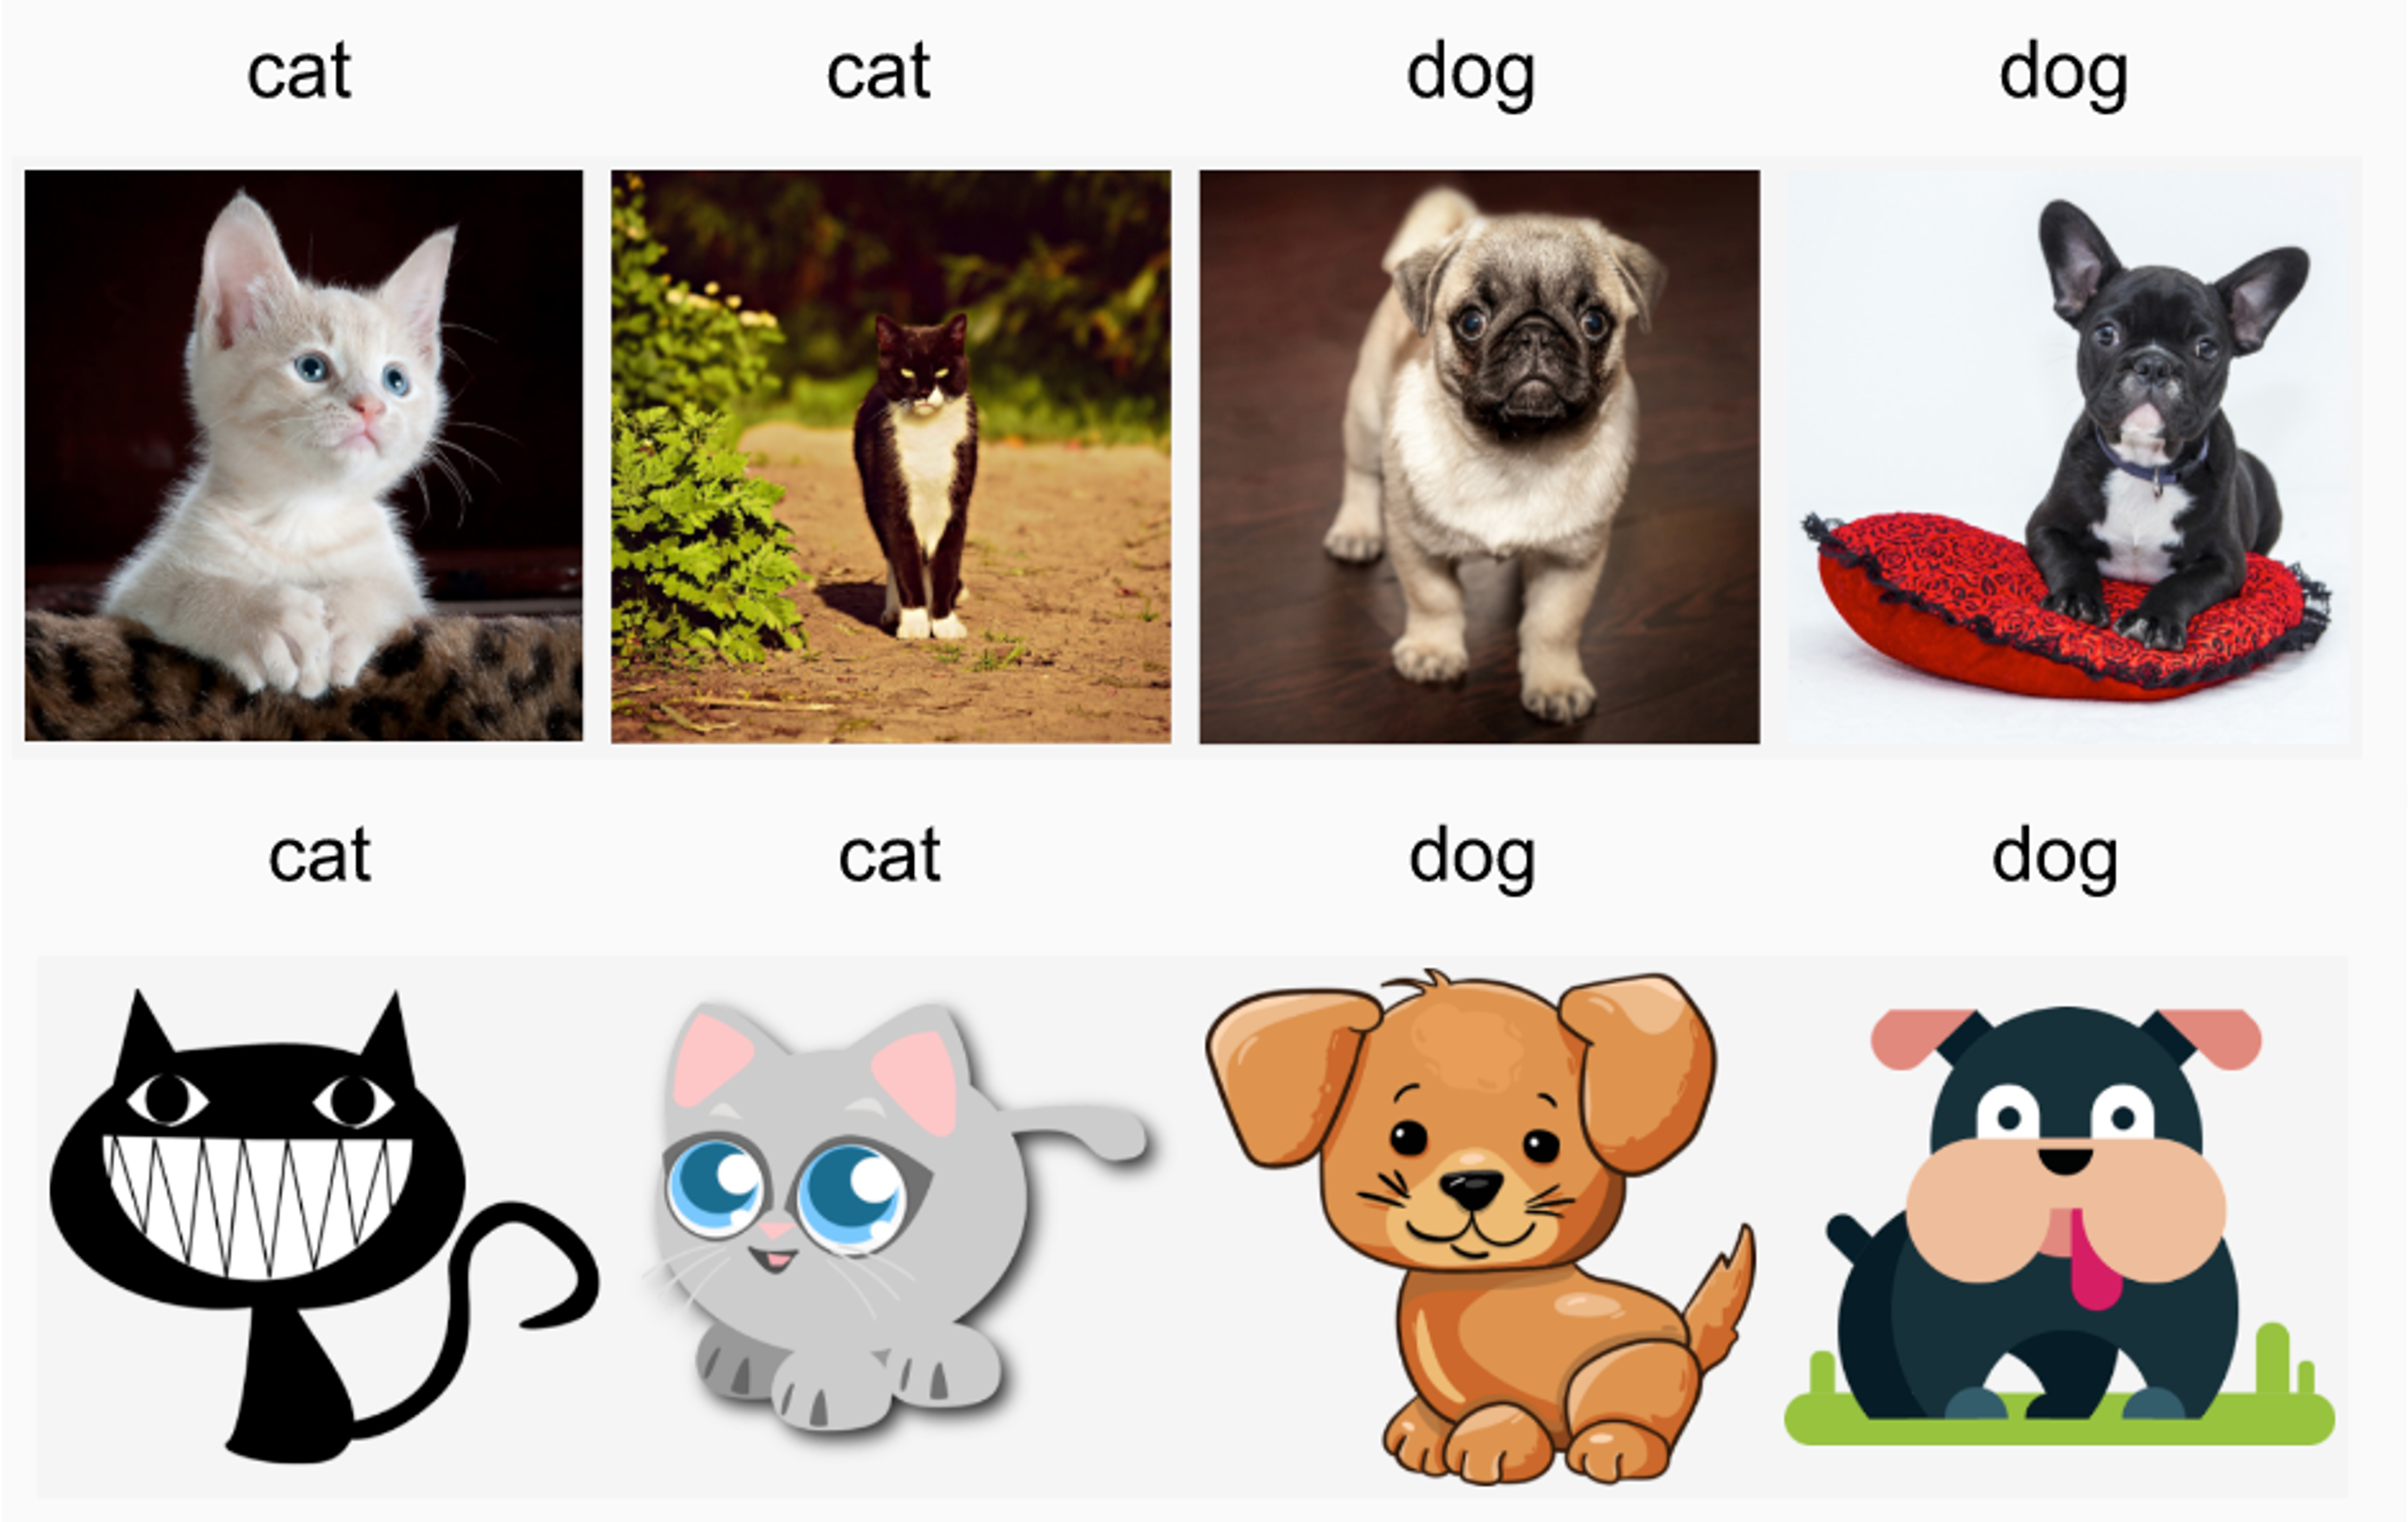
\includegraphics[width=13cm]{./images/catsanddogs} \caption{Two populations of cats and dogs potentially responsible for assuming overgeneralization}\label{fig:catsanddogs}
\end{figure}

\subsection{Accountability \& Transparency in AI:}\label{accountability-transparency-in-ai}

Transparency regarding AI refers to the quality of being open and explicit about how AI is developed and deployed and why.
Accountability refers to the fact or condition of taking responsible for ones action. Regarding AI, accountability discusses who should be held responsible for decisions that AI systems make.

Transparency and accountability are extremely difficult to address, mainly due to three reasons:

\begin{itemize}
\tightlist
\item
  Intentional Secrecy: Intentionally not revealing information that is hidden, for example, behind a business model or for reasons of natianal secuity;
\item
  Technical Illiteracy: People do not have the background knowledge and expertise to understand the language that AI developers use when communicating information for purposes of transparency and accountability;
\item
  Complexity of Infrastructure: AI algorithms may be difficult -or even- impossible to reverse engineer or to fully explain how and why the make specific decisions.
\end{itemize}

However, it is imperative - before deploying AI algorithms - to establish how they were conceived, with what intent, who sanctioned their implementation and who should be held responsible if they fail.

\subsection{Ethics and AIED}\label{ethics-and-aied}

Ethics can be understood as the moral principles that govern a person, a group of humans or extending to society. Ethical AI refers to the well-defined ethical guidelines regarding human values, such as human rights, non-discrimination, and privacy that AI systems should adhlere to.

Ethics for AIED, in particular, reflect the fundamental principles that AIED systems should respect and integrate by design. Among others, it is critical that AIED systems do not discriminate learners based on their background or characteristics, they respect learners' autonomy and agency, AIED systems should be transparent in terms of how they are implemented and how they make decisions while their decisions should be grounded on pedagogical reasoning, and they should promote societal and environmental well being.

Ethics in AIED is particularly critical today, also because it is not clear how AI can affect cognitive development of humans, especially minors. Therefore many international organizations such as the Council of Europe, UNESCO, and UNICEF have issued calls for evidence that demonstrate the impact of AI in education from the perspective of FATE, but also issue updates regarding ethical design and deployment of AIED.

\section{Questions for Chapter \ref{aied}}\label{questions-for-chapter-refaied}

\begin{enumerate}
\def\labelenumi{\arabic{enumi}.}
\tightlist
\item
  Please describe an application area of Artificial Intelligence in Education facing students and one facing teachers.
\item
  What are some ethical considerations for designing AI for learning? How could we address them?
\item
  What kind of computational methods are typically employed in AIED? Give examples.
\item
  They say that algorithms result in ``fair'' outcomes because they can't be biased, like humans. What is your opinion? Give an example of AI bias and explain how bias arises.
\end{enumerate}

\section{To-Read}\label{to-read-4}

\begin{enumerate}
\def\labelenumi{\arabic{enumi}.}
\tightlist
\item
  \href{https://www.researchgate.net/publication/241698223_What_is_AIED_and_why_does_Education_need_it}{What is AIED and why does Education need it?}
\item
  \href{https://www.buckingham.ac.uk/wp-content/uploads/2020/02/Summary-The-Institute-for-Ethical-AI-in-Educations-Interim-Report-Towards-a-Shared-Vision-of-Ethical-AI-in-Education.pdf}{The Institute for Ethical AI in Education Interim Report: Towards a Shared Vision of Ethical AI in Education}
\end{enumerate}

  \bibliography{book.bib,packages.bib}

\end{document}
